% To-Do List %
%   Chapter flow: intros and conclusions

\documentclass[11pt]{report}
\usepackage{StyleSheets/main}
\makeglossaries               % Only makes glossary in main file
\usetikzlibrary{external}     % Allows for cached complitation
\tikzexternalize[prefix=Graphs/tikz/] % Sets cache directory

\begin{document}
\documentclass[11pt]{report}
\usepackage{StyleSheets/main}
\usetikzlibrary{external}     % Allows for cached complitation
\tikzexternalize[prefix=Graphs/tikz/] % Sets cache directory

\begin{document}

\begin{titlepage}

    \tikzset{external/export next=false} % Exclude from externalization
    \begin{tikzpicture}[remember picture, overlay]
        \node[anchor=south east, inner sep=0, opacity=0.1, xshift=100mm, yshift=35mm] at (current page.south east) {
            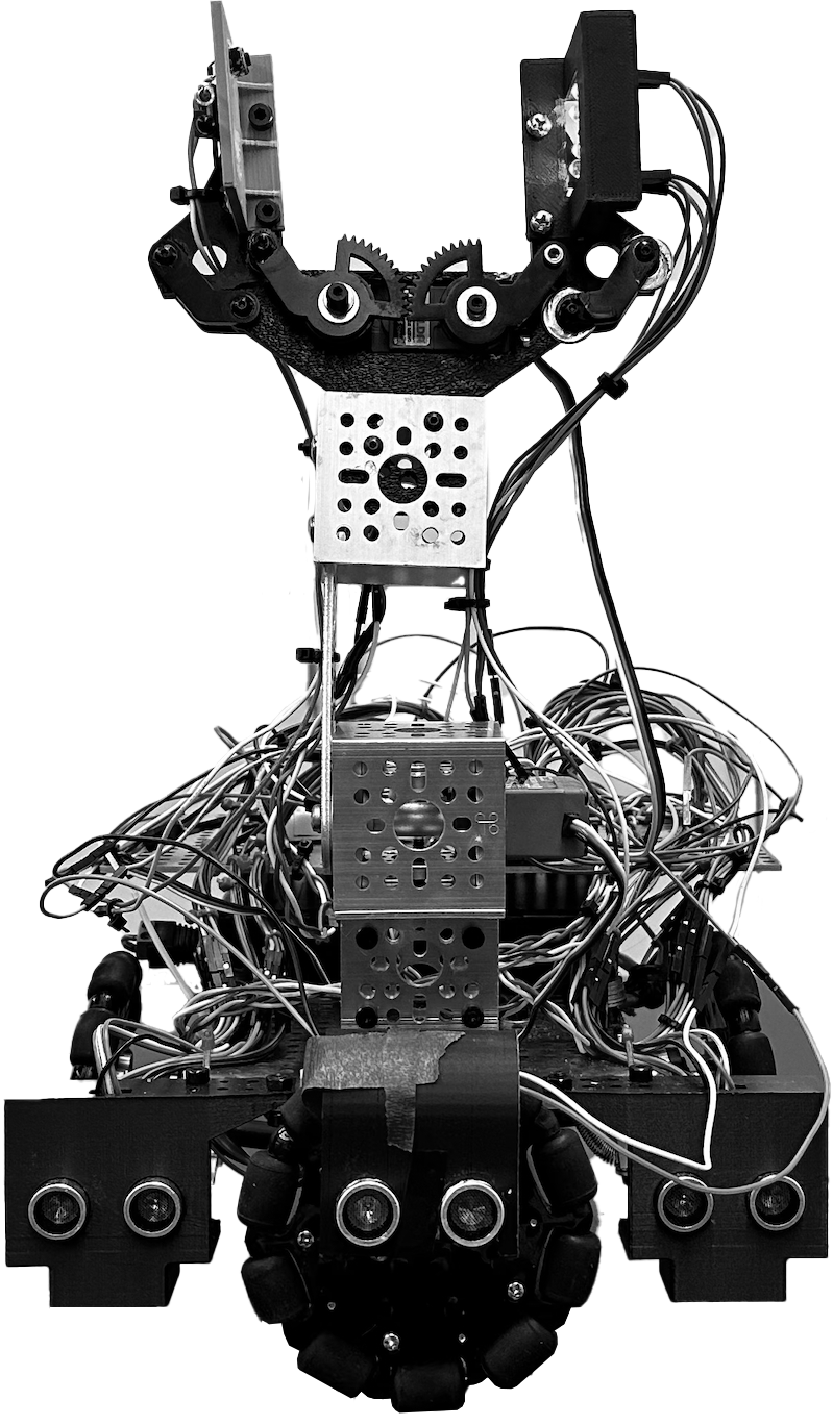
\includegraphics[width=\paperwidth]{Images/Robot/robot_front_view_greyscale.pdf}  % Adjust only width or height
        };
    \end{tikzpicture}
    
    \centering
    
    \Large{ENGR 2620}
    
    \Large{Integration II}
    
    \Large{Spring 2024}

    \vspace{0.5cm}
    
    \Huge \textsc{\TITLENAME}

    \vfill
    
    \vspace{1cm}
    
    \large{Dr. Jide Williams} \\
    \large{Dr. Irwin Jones}
    
    \vspace{0.8cm}

    \large \textbf{Prepared By:}
    \hspace{1.3cm} \begin{tabular}[t]{@{}l@{}}
        \textbf{Max Westerman}\\
        \textbf{Daniel Carey}\\
        \textbf{Charlie Buttrick}\\
        \textbf{Dylan Wright}\\
    \end{tabular}
    \vspace{10pt}
    
    \vfill
    \hfill \large Report Grade: \underline{\hspace{4cm}}
        
\end{titlepage}

\end{document}


    \begin{tikzpicture}[remember picture, overlay]
        \node[
            anchor=north west,
            fill=gray!20,
            minimum width=\paperwidth,
            minimum height=4cm,
            yshift=-17.35cm,
            xshift = 10.7cm
        ] at (current page.north west) {};
    \end{tikzpicture}

% ---------- %

\microtypesetup{protrusion=false} % Kerning disabled
\singlespacing
\tableofcontents
\listoffigures
\lstlistoflistings
\listoftables
\microtypesetup{protrusion=true} % Kerning Enabled

\newpage
\onehalfspacing

\documentclass[12pt]{report}
\usepackage{StyleSheets/main}
\begin{document}


\chapter{Introduction}\label{ch:introduction}
\onehalfspacing

Our project is about a vehicle (also referred to as a system) that has the ability to complete an obstacle course test as well as a pickup and placement test in a multitude of ways. On the obstacle course that is outlined by white lines on the side and green tape on the front and back end, our vehicle will be able to stay within the white lines and detect the walls within the course, maneuver around them, and stop on the green line at the end of the course. For the pickup and placement course, our vehicle will be able to detect an I-Beam, pick up a colored box, and based on its color and size, drop the box off on the other end of the course and return to the starting side of the court. Completing these tests requires communication skills, an array of engineering skills such as computer and electrical skills, writing skills, and decision-making skills. The project intends to strengthen all of the required skills needed to solve a complex problem that meets the demand being asked.

The purpose of the report is to detail the process of creating a system that will meet all requirements. The report was also a great way to get the team’s ideas flushed out and catch mistakes within our project that we could then correct. \Cref{ch:project-management-plan} keeps a timeline of the system’s progress by giving weekly updates that include the team member(s) who is responsible for the task and the duration of the task. Another key part of the report is \Cref{ch:system-requirements}. In this part of the report, the system requirements for certain objectives such as the obstacle avoidance and pickup and placement of the vehicle are established. Other major chapters of our report are \cref{ch:conceptual-design,ch:detailed-design}. \Cref{ch:conceptual-design} outlines the conceptual designs that the team came up and \cref{ch:detailed-design} details the design of the system which includes algorithms and other electrical and computer engineering tools that were used in the project. Lastly, \cref{ch:system-test} goes into depth about \gls{TEMPS}. In this chapter, an explanation of how each system requirement is tested is provided.

\end{document}
\documentclass[11pt]{report}
\usepackage{StyleSheets/main}

\begin{document}

\SectionuseSubSectionSizing
\SubSectionuseSubSubSectionSizing
\setlength{\parindent}{0pt} % Disables indentation

\chapter{Project Management Plan}\label{ch:project-management-plan}

\section{Week 1 (4/1/24 - 4/7/24)}
\subsection*{4/4}

\begin{itemize}
    \item Danny Carey and Charlie Buttrick looked over the provided kits and used the material checklist to verify all materials for the project were missing. \textbf{Duration: 50 minutes}
    \item Danny Carey and Charlie Buttrick test ultrasonic sensors. \textbf{Duration: 25 minutes}
\end{itemize}

\textbf{Week Summary:} Provided kits were checked and materials were verified. Ultrasonic Sensors were tested. Our objectives for next week will be to meet with Carter Sorenson and begin to talk about ideas for the obstacle test.

\section{Week 2 (4/8/24 - 4/14/24)}
\subsection*{4/8}

\begin{itemize}
    \item Danny Carey, Charlie Buttrick, and Max Westerman met to discuss the outline of the code. The idea to use classes was commonly agreed it would be most efficient due to making troubleshooting easier. \textbf{Duration: 25 minutes}
\end{itemize}

\subsection*{4/11}

\begin{itemize}
    \item Charlie Buttrick and Max Westerman met with Carter Sorenson for advice on the overall strategy of the project. The meeting also covered the subject of \gls{PID} controllers. \textbf{Duration: 60 minutes}
    \item Charlie Buttrick worked on pseudo-code for the obstacle test. \textbf{Duration: 1 hour and 30 minutes}
    \item Danny Carey began to work on the gripper, specifically a prototype design. \textbf{Duration: 1 hour}
    \item Danny Carey and Max Westerman brainstormed ideas for the overall design of the vehicle, with a targeted focus on wheel placement. \textbf{Duration: 1 hour}
\end{itemize}

\textbf{Week Summary:} The outline of the code was decided on. A project strategy was created, and \gls{PID} controllers were discussed. Pseudo-code written for obstacle test. A gripper prototype was designed. Wheel placement was discussed. Our objectives for next week will be to begin the design of the vehicle and simple movement testing.

\section{Week 3 (4/15/24 - 4/21/24)}
\subsection*{4/15}

\begin{itemize}
    \item Max Westerman worked on color sensors and added debug statements. \textbf{Duration: 35 minutes}
    \item Danny Carey and Max Westerman assembled wheels, motor controllers, and Teensy 4.1 board for design 1. \textbf{Duration: 1 hour and 45 minutes}
\end{itemize}

\subsection*{4/16}

\begin{itemize}
    \item Max Westerman ran a motor test for design 1. \textbf{Duration: 1 hour}
    \item Max Westerman tested the resistance of black and silver screws that will be used to connect the battery and motor controller. \textbf{Duration: 25 minutes}
\end{itemize}

\subsection*{4/18}

\begin{itemize}
    \item Danny Carey continued work on the gripper arm and began to add wiring. \textbf{Duration: 1 hour and 30 minutes}
    \item Charlie Buttrick and Max Westerman brainstormed ideas for code of the obstacle course and the location of the ultrasonic sensors on the vehicle. \textbf{Duration: 1 hour}
    \item Charlie Buttrick and Max Westerman thought of ideas to fix side wheels that were stalling on forward movement. \textbf{Duration: 30 minutes}
\end{itemize}

\textbf{Week Summary:} Debug statements added to code. Wheels assembled with motor controllers and Teensy 4.1 for design 1. Motor test conducted. Resistance of screws tested for battery connection. Gripper wiring added. Obstacle code and ultrasonic sensor location discussed. Ideas to fix side wheels that were stalling generated. Our objectives for next week will be to work on our detailed design presentation and continue to build system, specifically the placement of the ultrasonic sensors.

\section{Week 4 (4/22/24 - 4/28/24)}
\subsection*{4/23}

\begin{itemize}
    \item Danny Carey and Charlie Buttrick began to work on detailed design review. \textbf{Duration: 1 hour}
    \item Charlie Buttrick focused more on customer requirements, the project management plan, the purpose, and the current state of the project.
    \item Danny Carey focused on the project design outline, the design matrix, and the current state of the project.
\end{itemize}

\subsection*{4/25}

\begin{itemize}
    \item Danny Carey and Charlie Buttrick moved ultrasonic sensors to the front of the vehicle. \textbf{Duration: 35 minutes}
    \item Danny Carey and Charlie Buttrick added washers to the side wheels to try to fix the side wheels from stalling. \textbf{Duration: 30 minutes}
    \item Danny Carey and Charlie Buttrick took apart Design 1, specifically the wiring and placement of the battery. The motor controllers and wheels are still intact. \textbf{Duration: 35 minutes}
    \item Dylan Wright, Danny Carey, and Charlie Buttrick gave detailed design review presentation.
\end{itemize}

\textbf{Week Summary:} Detailed design review started. Ultrasonic sensors are placed in front of vehicles. Washers were placed under side wheels to try to fix stalling. Design 1 deconstructed (wiring/battery). Detailed design presentation takes place and feedback is given. Our objectives for next week will be to begin writing the obstacle code and discuss the line following code.

\section{Week 5 (4/29/24 - 5/5/24)}
\subsection*{4/30}

\begin{itemize}
    \item Charlie Buttrick and Max Westerman met to discuss and begin code for obstacle course test, specifically adding classes to the code for more scenarios. \textbf{Duration: 1 hour}
    \item Charlie Buttrick and Max Westerman discussed the line following code. \textbf{Duration: 30 minutes}
\end{itemize}

\subsection*{5/2}

\begin{itemize}
    \item It was discovered that after Design 1 was taken apart, multiple wire tips were disconnected and broken. \textbf{Duration: 2 hours}
    \item Charlie Buttrick tried to solder back one wire to the motor and accidentally burned the motor. The team bought a new motor.
    \item Max used equipment in the innovation lab to solder back the wires to the motors and motor controllers.
    \item Charlie Buttrick added to the ultrasonic code. \textbf{Duration: 1 hour}
    \item Danny Carey began to build Design 2, focused on the placement of the battery and Teensy 4.1 board. Also, added wiring for the Teensy 4.1 board and battery. \textbf{Duration: 1 hour and 30 minutes}
\end{itemize}

\textbf{Week Summary:} Obstacle avoidance and line following code discussed. Multiple damages and breakages were discovered after Design 1 was deconstructed. Soldering was attempted but the motor broke. New motor was burnt and the innovation lab was used to solder wires. Ultrasonic code improved. Design 2 was built, battery placement and Teensy 4.1 placement and wiring focus. Our objectives for next week will be to test our obstacle avoidance code and make progress with building the gripper. Another objective will be to complete the gripper wiring for the gripper and test design 2 on the obstacle course.

\section{Week 6 (5/6/24 - 5/12/24)}
\subsection*{5/7}

\begin{itemize}
    \item Charlie Buttrick, Danny Carey, and Max Westerman combined the motor controller plate and battery/Teensy 4.1 board plate. \textbf{Duration: 30 minutes}
    \item Charlie Buttrick, Danny Carey, and Max Westerman placed sensor mounts on the front of the vehicle and attached ultrasonic sensors. \textbf{Duration: 30 minutes}
    \item Charlie Buttrick and Max Westerman verified the ultrasonic sensor code. \textbf{Duration: 25 minutes}
\end{itemize}

\subsection*{5/9}

\begin{itemize}
    \item Charlie Buttrick, Danny Carey, Dylan Wright, and Max Westerman tested the obstacle test. \textbf{Duration: 1 hour and 40 minutes}
\end{itemize}

\subsection*{5/10}

\begin{itemize}
    \item Danny Carey and Max Westerman completed the wiring for the gripper. \textbf{Duration: 1 hour and 40 minutes}
\end{itemize}

\subsection*{5/12}

\begin{itemize}
    \item Charlie Buttrick and Max Westerman tried to fix the side wheels' stalling issue by adding heavy mass to the vehicle. \textbf{Duration: 1 hour and 30 minutes}
    \item Charlie Buttrick, Danny Carey, and Max Westerman decided to take apart Design 2.
    \item Danny Carey builds customized sensor mounts in SolidWorks. \textbf{Duration: 1 hour}
    \item Max Westerman takes apart all of Design 2 except the motor controller and wheel placement and wires. \textbf{Duration: 1 hour}
    \item Charlie Buttrick and Max Westerman think about the idea of IR sensors. \textbf{Duration: 35 minutes}
\end{itemize}

\textbf{Weekly Summary:} Motor controller plate and battery/Teensy 4.1 plate combined. Sensor mounts and ultrasonic sensors are attached. Ultrasonic sensor code verified. Obstacle course run tested. Wiring for gripper completed. Heavy mass was added to the vehicle to fix the side wheels stalling. Design 2 taken apart. Customized sensor mounts built in SolidWorks. \gls{IR} sensor idea discussed. Our objectives for next week will be to test redesign Design 3 as well as test the gearboxes to see if they will or will not impact the speed. Also, sensor mounts will be printed for the ultrasonic sensors. We will also want to finish the line following code and begin testing and implement the \gls{IR} Array.

\section{Week 7 (5/13/24 - 5/19/24)}
\subsection*{5/13}

\begin{itemize}
    \item Danny Carey 3-D prints sensor mounts for Design 3. \textbf{Duration: 10 minutes}
    \item Max Westerman tests the compatibility of gearboxes for torque motors. It is deemed successful thus 2 motors of the vehicle are replaced. \textbf{Duration: 30 minutes}
    \item Max Westerman machined down a dead torque motor gearbox. This verified that the torque motor would be faster when modified. \textbf{Duration: 3 hours}
\end{itemize}

\subsection*{5/14}

\begin{itemize}
    \item Danny Carey and Max Westerman assembled Design 3, the plate with the motor controllers and wheels are attached to the plate with the Teensy 4.1 board as well as the battery. \textbf{Duration: 2 hours and 30 minutes}
\end{itemize}

\subsection*{5/16}

\begin{itemize}
    \item Danny Carey attaches the customized sensor mounts to the vehicle and the color and ultrasonic sensors are attached. \textbf{Duration: 40 minutes}
    \item Charlie Buttrick, Dylan Wright, Danny Carey, and Max Westerman test Design 3 on the obstacle test. \textbf{Duration: 1 hour and 30 minutes}
    \item Charlie Buttrick and Max Westerman test the basic line following code. \textbf{Duration: 35 minutes}
    \item Danny Carey designed a sensor mount for the bottom of the vehicle. \textbf{Duration: 1 hour}
\end{itemize}

\subsection*{5/19}

\begin{itemize}
    \item Danny Carey and Max Westerman attach the gripper to the vehicle. \textbf{Duration: 1 hour}
    \item Danny Carey and Max Westerman attach an \gls{IR} array and color sensor to the sensor mount on the bottom of the vehicle. \textbf{Duration: 1 hour and 30 minutes}
\end{itemize}

\textbf{Week Summary:} Sensor mounts for Design 3 printed. Compatibility of gearboxes for torque motors tested. 2 motors are replaced. Design 3 is assembled. Sensor mounts are attached. Design 3 tested on an obstacle test. Basic line following code tested. Sensor mount for bottom of vehicle designed. Gripper attached to the vehicle. \gls{IR} and color sensor attached to the vehicle. Our objectives for next week will be to clean up the wiring of the system, add pushbuttons to the end of the gripper arm, continue obstacle testing, test the line following code and improve the vehicle’s ability to follow the line as needed.

\section{Week 8 (5/20/24 - 5/26/24)}
\subsection*{5/20}

\begin{itemize}
    \item Danny Carey and Max Westerman rewired the color sensors, the gripper, the \gls{IR} array, and the ultrasonic sensor. \textbf{Duration: 1 hour and 20 minutes}
    \item Danny Carey and Max Westerman implemented, coded, and wired the button toggle for the gripper. \textbf{Duration: 30 minutes}
    \item Danny Carey and Max Westerman secured the plastic gripper gear via reversible super glue and lock tight. \textbf{Duration: 1 hour and 30 minutes}
    \item Max Westerman coded the gripper pick-up and place schema and tested. \textbf{Duration: 1 hour}
    \item The middle color sensor is burnt.
    \item Max Westerman tested obstacle avoidance. \textbf{Duration: 2 hours}
    \item Max Westerman designed and implemented a suspension system on the vehicle. \textbf{Duration: 3 hours}
\end{itemize}

\subsection*{5/21}

\begin{itemize}
    \item Max Westerman implemented the suspension system. \textbf{Duration: 1 hour and 25 minutes}
    \item Max Westerman and Charlie Buttrick began to code the \gls{IR} array algorithm as well as brainstorm how to implement \gls{PID} logic. \textbf{Duration: 1 hour}
    \item Max Westerman worked on pick-up and placement code for the system. \textbf{Duration: 1 hour and 10 minutes}
    \item Danny Carey redesigned sensor mounts for the front of the vehicle after it was discovered it cracked. \textbf{Duration: 45 minutes}
    \item Max Westerman and Charlie Buttrick worked on and tested the line following code. \textbf{Duration: 2 hours}
    \item Danny Carey replaced the middle burnt color sensor. \textbf{Duration: 25 minutes}
\end{itemize}

\subsection*{5/22}

\begin{itemize}
    \item Danny Carey designed a mount for the end of the gripper arm via SolidWorks. \textbf{Duration: 1 hour}
    \item Danny Carey and Max Westerman continued to wire the gripper as sensors and pushbuttons were being added. \textbf{Duration: 2 hours}
\end{itemize}

\subsection*{5/23}

\begin{itemize}
    \item Danny Carey and Charlie Buttrick attached a new sensor mount to the bottom side of the front end of the vehicle. \textbf{Duration: 1 hour}
    \item Max Westerman color-calibrated the \gls{IR} array and updated the code. \textbf{Duration: 1 hour and 30 minutes}
    \item Max Westerman wired the sensor mount on the bottom side of the front end of the vehicle. \textbf{Duration: 25 minutes}
    \item Max Westerman added a vertical box length variable to the pickup and placement code to help center the vehicle. \textbf{Duration: 15 minutes}
    \item Max Westerman improved the color sensor calibration for the front-end sensors of the vehicle. \textbf{Duration: 25 minutes}
\end{itemize}

\subsection*{5/24}

\begin{itemize}
    \item Max Westerman completed the \gls{IR} array code with a calibrated error. \textbf{Duration: 45 minutes}
    \item Max Westerman tested the \gls{IR} array code to make sure if the vehicle deviates from the line, it will correctly realign with the line. \textbf{Duration: 1 hour}
    \item Max Westerman added an \gls{LED} feature that connects to the battery being turned on. \textbf{Duration: 45 minutes}
\end{itemize}

\textbf{Week Summary:} Gripper, color sensors, \gls{IR} array, and ultrasonic sensor rewired. A pushbutton for the gripper was added, wired, and coded. The \gls{IR} array was tested and completed. Our objectives for next week will be to test the gripper arm and test the full pick up and placement course.

\section{Week 9 (5/27/24 - 6/2/24)}
\subsection*{5/27}

\begin{itemize}
    \item Max Westerman and Danny Carey test gripper arm. \textbf{Duration: 2 hours}
    \item Danny Carey designs a sensor mount for the ultrasonic sensor that will be put on the front of the vehicle. \textbf{Duration: 1 hour}
\end{itemize}

\subsection*{5/28}

\begin{itemize}
    \item Max Westerman and Charlie Buttrick calibrate and wire the ultrasonic sensor and mount the sensor mount as well as add the ultrasonic sensor to the mount. \textbf{Duration: 1 hour}
    \item Max Westerman, Danny Carey, and Charlie Buttrick test the full line following and pickup and placement test. \textbf{Duration: 1 hour and 45 minutes}
\end{itemize}

\subsection*{5/30}

\begin{itemize}
    \item Charlie Buttrick, Danny Carey, Max Westerman, and Dylan Wright test vehicle on obstacle course and the test is deemed complete.
    \item Charlie Buttrick, Danny Carey, Max Westerman, and Dylan Wright brainstorm ideas of how to fix the pickup and place test which is stemming from an ultrasonic sensor issue. \textbf{Duration: 30 minutes}
\end{itemize}

\subsection*{6/2}

\begin{itemize}
    \item Charlie Buttrick, Danny Carey, and Max Westerman improve color calibration of all sensors and alter ultrasonic sensor code. \textbf{Duration: 2 hours and 30 minutes}
    \item Danny Carey and Max Westerman test line following and pick up and placement test and were able to get consecutive successful tests. \textbf{Duration: 1 hour}
\end{itemize}

\textbf{Week Summary:} The gripper arm is tested and the tests are deemed successful. An ultrasonic sensor is added. The obstacle test was completed. Our objectives for next week will be to test the pickup and placement test to get a complete test.

\section{Week 10 (6/3/24 - 6/9/24)}
\subsection*{6/3}

\begin{itemize}
    \item Charlie Buttrick, Danny Carey, Max Westerman, and Dylan Wright test vehicle on line following and pickup and placement course and the test is deemed complete.
    \item Danny Carey and Dylan Wright take apart vehicle. \textbf{Duration: 25 minutes}
\end{itemize}


\SectionuseNormalSectionSizing
\SubSectionuseNormalSectionSizing

\end{document}
\documentclass[11pt]{report}
\usepackage{StyleSheets/main}
\begin{document}

\chapter{System Requirements}\label{ch:system-requirements}

The overall objective of the system our team has built involves numerous requirements that helped us achieve our objectives. One of the main goals will be for the vehicle to complete the obstacle course in a timely fashion that avoids walls and does not pass specific colored tape. The other main goal will be for the obstacle to pick up a specific colored box, and then follow a particular line of color of the box to a drop-off site, where the vehicle will place the box back down.

\section{Box Pick-up and Placement System}

\subsection{Recognition of the I-Beam}
The vehicle shall find the I-Beam on the course.

\subsection{Orientation of the I-Beam}
The vehicle shall orientate/center itself with the I-Beam

\subsection{Apprehend the Box}
The vehicle shall apprehend the box with the gripper.

\subsection{Identify the Color of the Box}
The vehicle shall identify the color of the box.

\subsection{Identify the Size of the Box}
The vehicle shall identify the size of the box. 

\subsection{Realign with the Line Following Course}
The vehicle shall move itself back onto the line following the course after it has apprehended the box.

\subsection{Follow the Line of the Color of the Box and Return.} 
The vehicle shall follow the colored line of the box’s color it has apprehended.

\subsection{Placement of the Box}
The vehicle shall place the box on the appropriate I-Beam based on the color and size of the box.

\section{Drive Train \& Steering System}

\subsection{Move Forward}
The vehicle shall move forward in a straight line.

\subsection{Move Backward}
The vehicle shall move backward in a straight line.

\subsection{Move Right}
The vehicle shall move right in a straight line.

\subsection{Move Left}
The vehicle shall move left in a straight line.

\subsection{Rotational Movement}
The vehicle shall rotate to the right or left.

\section{Sensor Requirement: IR Sensor Array}

\subsection{Width of the IR Sensors}
The width of the \gls{IR} Array shall be bigger than the width of the tape.

\subsection{The number of sensors is greater than 6}
The amount of sensors on the \gls{IR} Array is greater than 6.

\subsection{It Must Detect and Distinguish the Tape and Tarp}
The \gls{IR} Array must be able to distinguish between the colored tape and the black tarp.

\subsection{It Must be able to Calculate Error}
The \gls{IR} Array must be able to calculate the error to recognize which way the vehicle is deviating.

\subsection{Deviation Adjustment}
The vehicle shall properly correct the vehicle if it deviates from the red, blue, or green line.

\section{Task-2 Completion Times (Obstacle Course)}

\subsection{Detection of Walls }
The vehicle shall detect the walls of the obstacle course via ultrasonic sensors
\subsection{Avoidance of Walls}
The vehicle shall move forward and avoid the walls of the obstacle course by the system not touching any part of the wall. 

\subsection{Detection of Side Boundaries of Obstacle Course via Color Sensors}
The vehicle shall have color sensors that will identify when the system is at the side boundaries of the course. For this specific test, the side boundary is outlined by white tape.

\subsection{Stay within the Obstacle Course Until Course is Complete}
The vehicle’s center of mass shall not deviate outside the side boundary and stay within the obstacle course until completion. 

\subsection{Detection of the Finish Line of Obstacle Course via Color Sensors}
The vehicle shall have color sensors that will identify when the system is at the side boundaries of the course. For this specific test, the side boundary is outlined by white tape.

\subsection{System Stops at the End of the Course}
The vehicle shall detect the green line and fully cross the line, and then stop. 


\end{document}
\documentclass[11pt]{report}
\usepackage{StyleSheets/main}
\begin{document}

\chapter{CONOPs (Concept of Operations)}\label{ch:conops}
The purpose of this section is to provide the user of the robot with a clear and concise description of how this system is operated. The \gls{CONOP}s provides a clear summary of how the vehicle will reach it's objective. 
\section{System Summary}
\begin{itemize}
    \item This system is a vehicle with the ability to move right, left, forwards, backwards, and rotate. This vehicle is powered by a battery and controlled using a microcontroller.
    \item The vehicle has a gripper with an arm that allows it to reach for \& pick up objects. 
    \item This vehicle can detect colors, obstacles, and lines.
\end{itemize}
\section{Initialization of the System}
\begin{itemize}
    \item Firstly, the \gls{ABHS} will be placed down on a flat surface, preferably the floor as it takes away the risk of the vehicle falling from a dangerous height.
    \item If the use of the \gls{ABHS} is to fulfill one of its requirements (Obstacle Avoidance, Pickup and Place System with Line Following), then the \gls{ABHS} should be placed in its starting position.
    \item All the connections should be secure and in accordance with the pin map provided with the vehicle.
    \item If a new version of the code is uploaded, verify that the \texttt{while (!Serial)} portion of the \cref{lst:main-h} has been commented out.
    \item Ensure that any external connections the the Teensy 4.1 are terminated to eliminate the possibility of over-powering the Teensy 4.1.
    \item The battery should at this point be connected and switched on, with the green lights appearing when the battery is on. The additional blue \gls{LED} will also light up when the battery is turned on.
\end{itemize}

\section{Standard Operating Modes}
\begin{itemize}
\item This system has 2 normal operating modes:
    \begin{itemize}
        \item This system was designed to perform obstacle avoidance. In the event of a wall being placed in front of the system, the vehicle would find a way around the wall as long as white boundary lines outline the obstacle course.
        \item This system was designed to pick up a box and recognize its color. It will then use this color to transport the box over a line of the same color, and place it in the platform dependant on the size of the box/package. It will then return to its starting position.
\end{itemize}
\end{itemize}
\section {External Environment for use of the System}
\begin{itemize}
    \item This system should typically be used in a room temperature, dry environment. This is due to the open wire nature of the \gls{ABHS}, and its use-case of clean-room operation.
\end{itemize}
\section{Standard Maintenance}
\begin{itemize}
    \item The battery for the \gls{ABHS} should always be charged in order for this system to work.
    \item All wires should be maintained in the correct pin ports. If a wire is in the incorrect port, follow the provided pinout \cref{fig:Pinoutmap}.
    \item The vehicle should be kept in dry, stable conditions, and out of direct sunlight as to avoid potential damage to parts.
\end{itemize}
\section{Failure Modes due to Internal Problems}
\begin{itemize}
    \item In the event of the user at any point seeing or smelling smoke coming from the vehicle, shut the battery off as soon as possible. 
    \item In the case of these events, troubleshoot the system to decipher what the problem point was. Start by seeing if any parts of the system are hot, specifically motors, the Teensy 4.1 microcontroller, and the buck converter. If any signs of overheating occur, immediately disconnect the part for further inspection.
    \item Test the possibly damaged component to see if it functions correctly, if not, replace the damaged component.
\end{itemize}
\section{Reaction to External Failure Modes}
\begin{itemize}
    \item If on the obstacle course the vehicle drives into one of the walls, it should find its own way around it. 
    \item If the vehicle exits the testing course, (ie. over the white line), immediately switch the battery off to avoid the vehicle running too far off course \& potentially crashing, damaging the vehicle.
    \item If during the box pickup test the vehicle drops the box, reset the course and try to run the system again. If this fails again, check to ensure that the gear teeth of the gripper are properly connected.
    \item If the vehicle fails to follow the line and veers off the path, turn off the battery and reset the course. 
\end{itemize}
\section{Shutdown of the System}
\begin{itemize}
    \item Make sure the vehicle has fully run the course of its current objective. Turn the battery off and ensure that the system is fully off. If the vehicle is acting erroneously, it can be manually shut off during it's operation, as it is minimally hazardous to operators.
\end{itemize}


\end{document}
\documentclass[11pt]{report}
\usepackage{StyleSheets/main}
\begin{document}

\chapter{Conceptual Design}\label{ch:conceptual-design}

\section*{Design Strategy}
Before the initial design process had begun, it was clear to the team that there would be a trade-off between complexity and efficiency - as such, it was determined that the complexity of the system would have to increase greatly in order to get the maximum potential performance from the robot. The following designs are variations of the previous, with each design increasing in complexity.
\par Other teams reduced the amount of electrical components that connected to the Teensy 4.1 microcontroller to reduce the complexity of the code base, seen in \cref{ap:code}. This did not influence the design of this robot as the code base was designed from the ground up to be a modular system, utilizing an object oriented approach in \cplusplus{}, ensuring no extra code needed to be written or maintained the more sensors were added to the cart. Consequently, the design process was unrestricted by the quantity or variety of sensors available, permitting a more flexible approach to design.

\subsection*{Abbreviations used in Drawings}
\begin{itemize}
    \item \gls{US}
    \item \gls{CS}
    \item \gls{IRS}
    \item \gls{omni}
    \item \gls{FS}
    \item \gls{B}
\end{itemize}

\newpage
\section{Design 1}\label{sec:design1}
\begin{figure}[H]
    \centering
    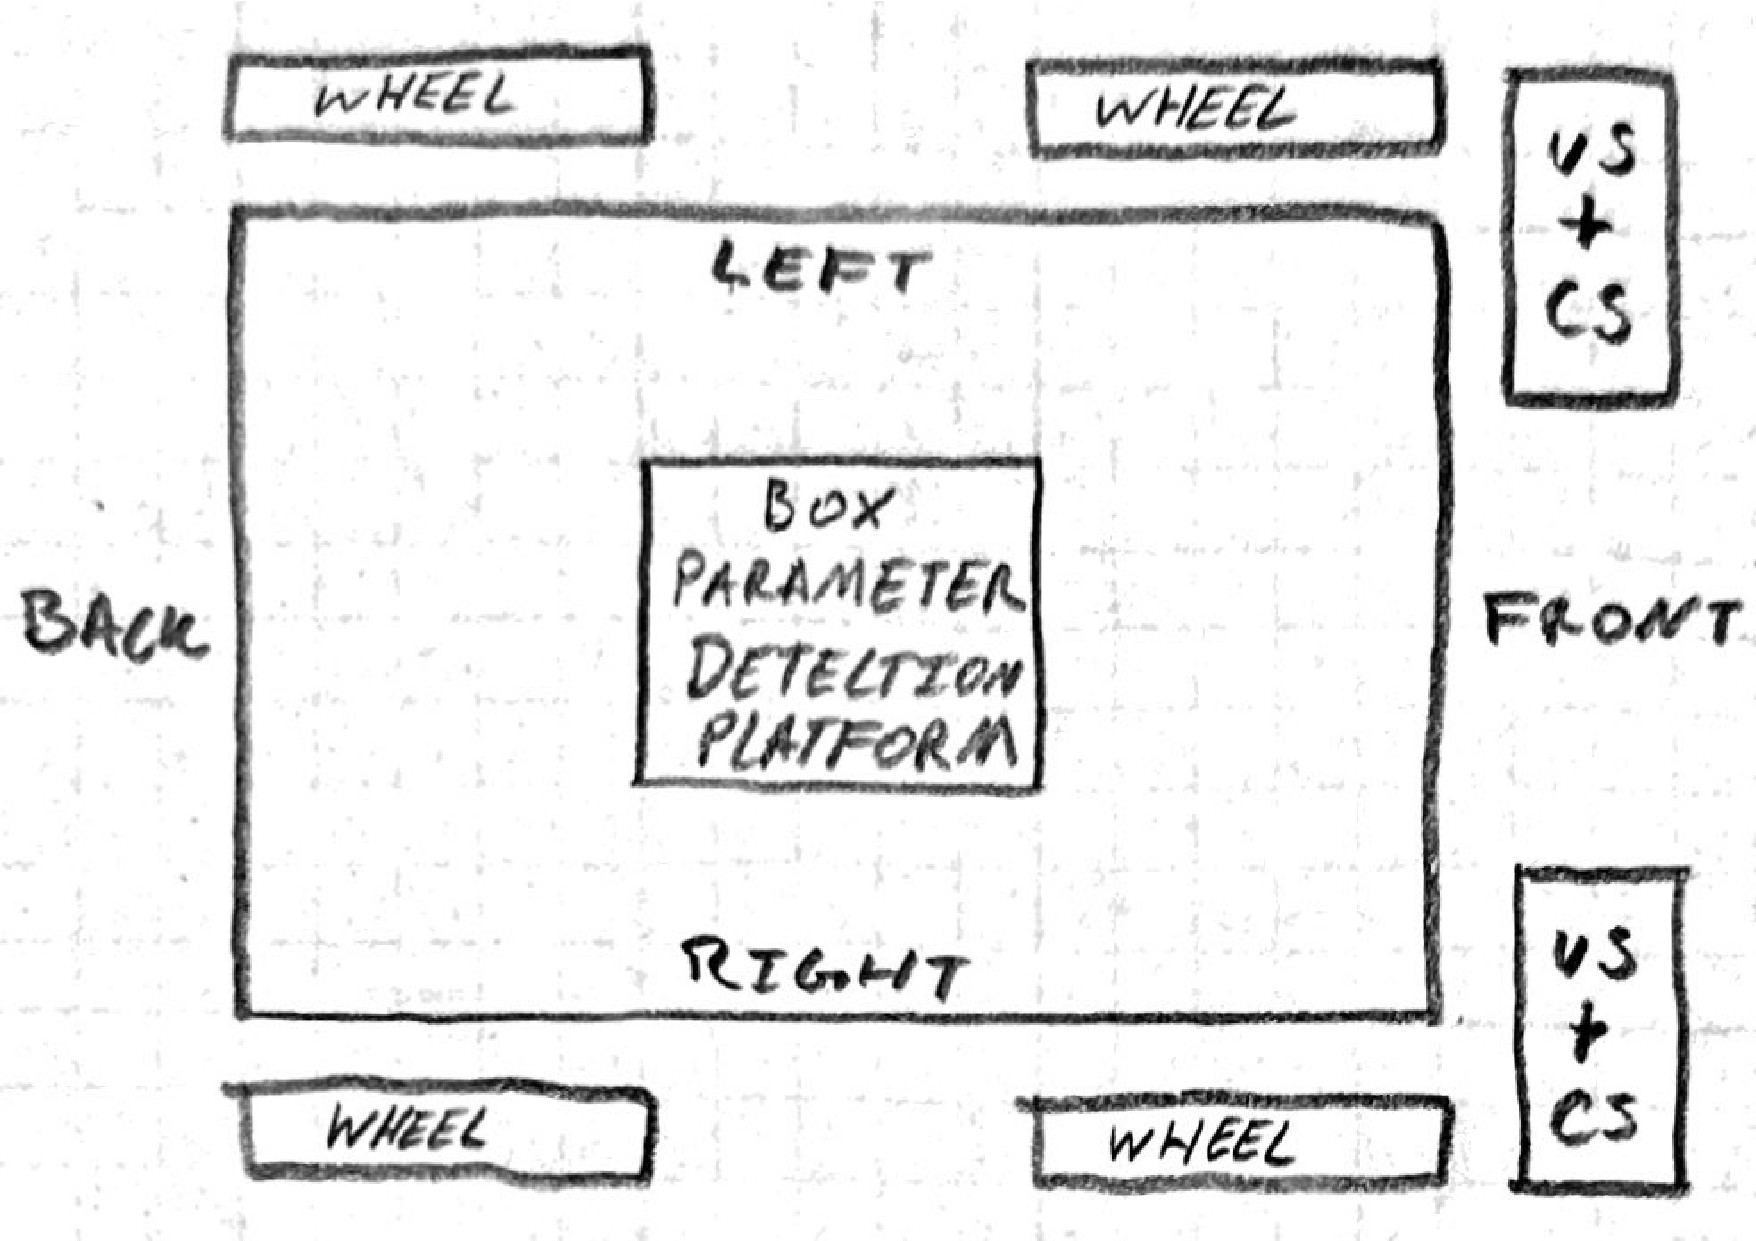
\includegraphics[width=0.5\linewidth]{Images//Designs/Design1a.pdf}
    \caption{Design 1a - simplified layout of movement and sensor systems}
    \label{fig:design1a}
\end{figure}
The first design is an adaptation of the fundamental designs demonstrated throughout the prerequisite course, Integration I, for the sake of setting a baseline. Efficiency and speed are sacrificed for simple movement and sensor algorithms.

\begin{description}
    \item[Wheel Configuration --] This design utilizes a standard 2x2 wheel configuration featuring standard 1 \gls{DoF} wheels. This configuration performed consistently, yet was problematic when it came to creating highly dynamic movement algorithms.
    %
    \item[Sensor Configuration --] The front corners are fitted with dual-purpose sensor mounts, containing both an \gls{RGB} color sensor and an ultrasonic sensor to be used for all spatial objectives: line following, boundary/obstacle/object detection, and directional orientation.
\end{description}

\begin{figure}[H]
    \centering
    \hspace*{6em}
    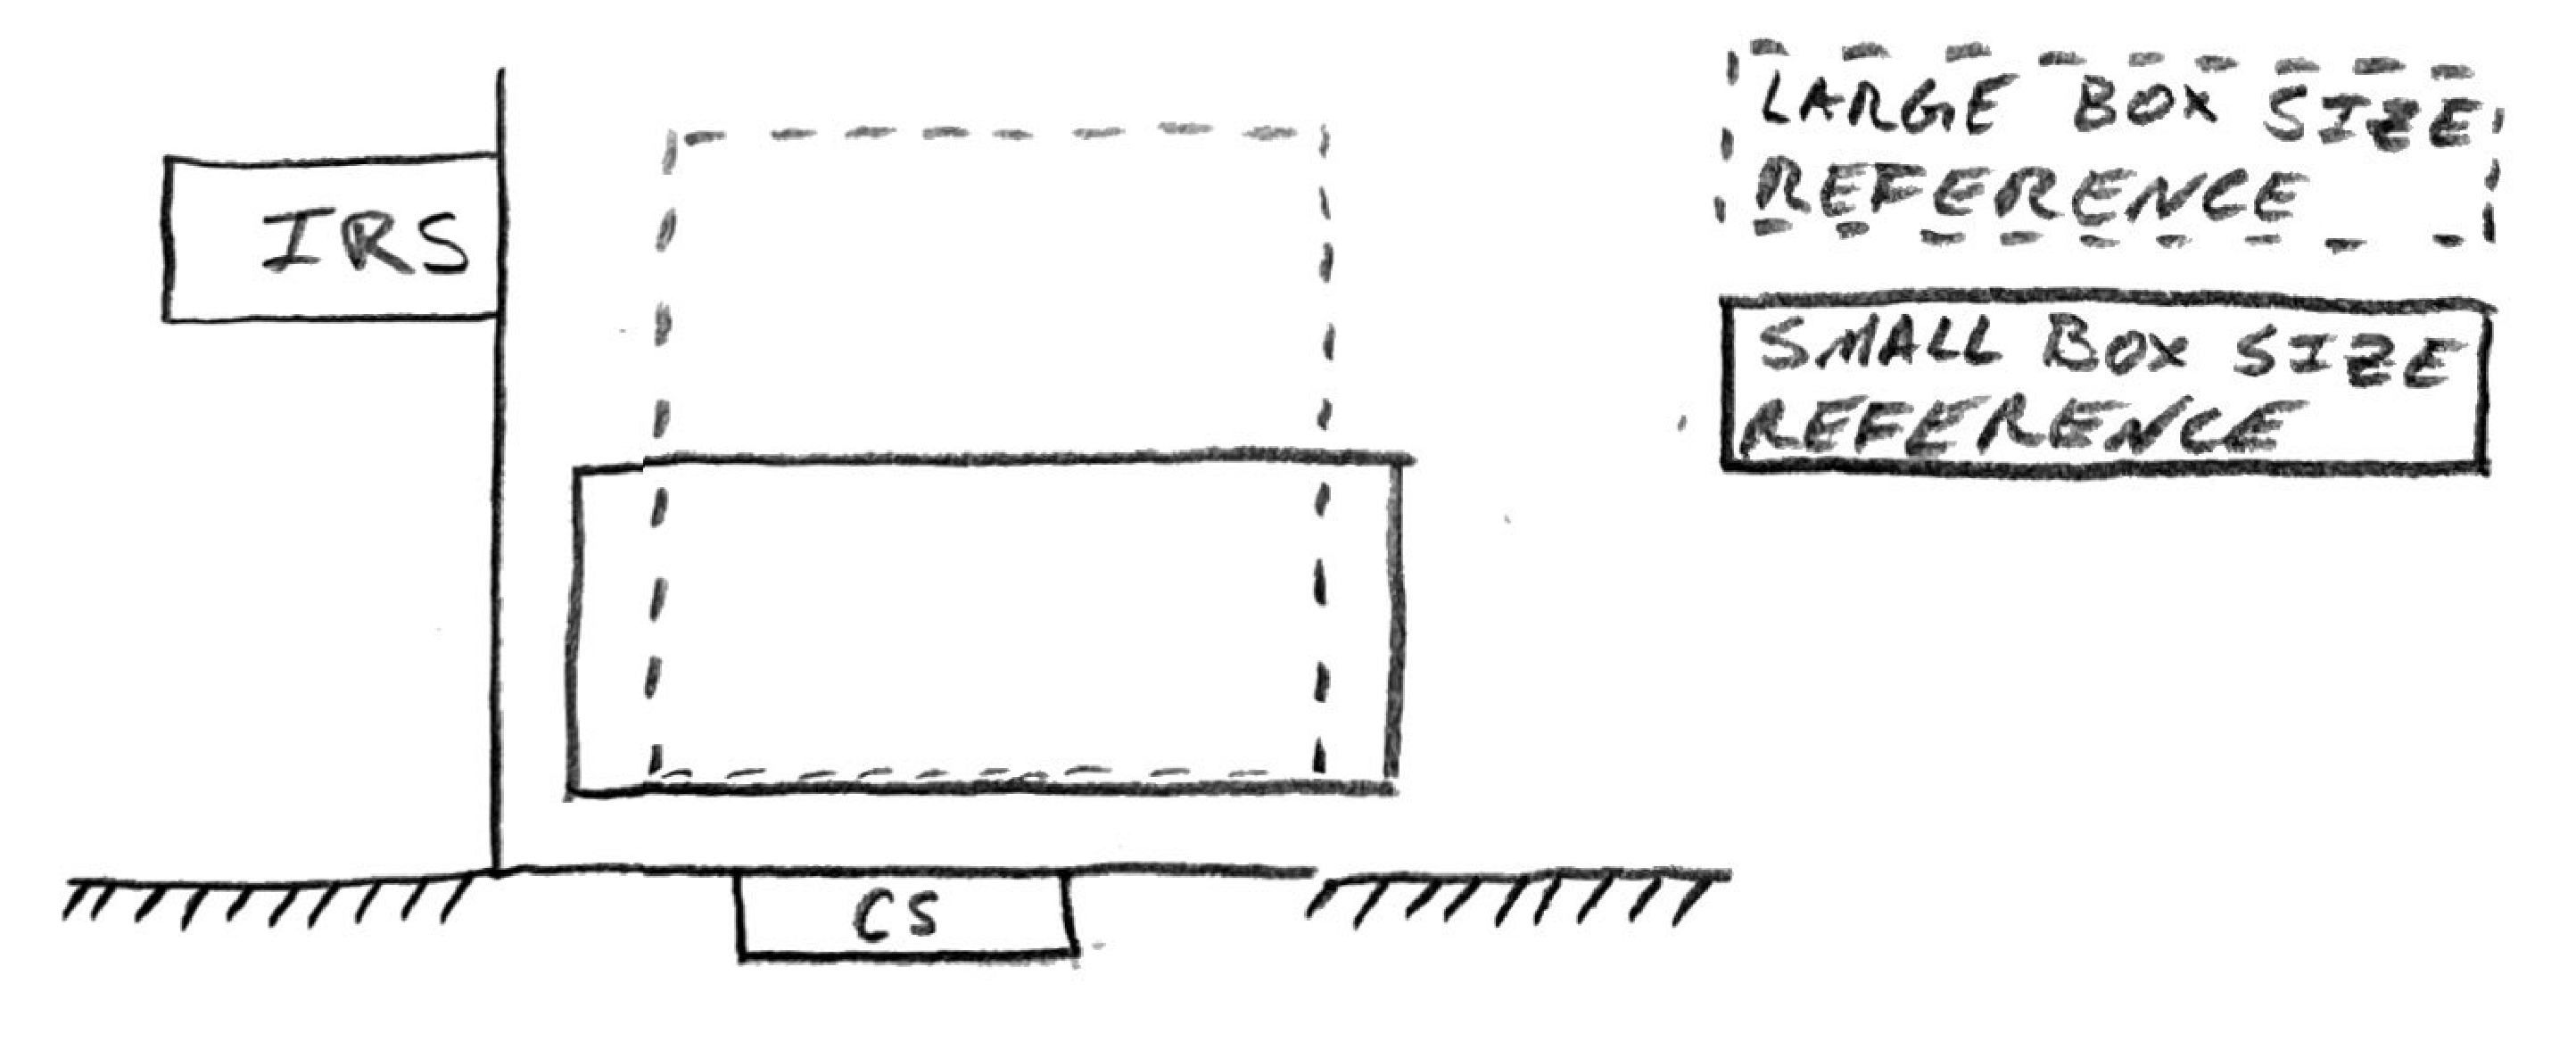
\includegraphics[width=0.6\linewidth]{Images//Designs/Design1b.pdf}
    \caption{Design 1b - Box property detection platform with \gls{IRS}}
    \label{fig:design1b}
\end{figure}
\begin{description}
    \item[Box Property Detection --]A gripper mechanism is to place the box onto a small platform on top of the robot that will contain an \gls{RGB} sensor to determine the package color, alongside an infrared sensor placed high enough to only detect the larger of two possible box sizes.
\end{description}

\newpage
\section{Design 2}\label{sec:design2}
\begin{figure}[H]
    \centering
    \hspace*{2em}
    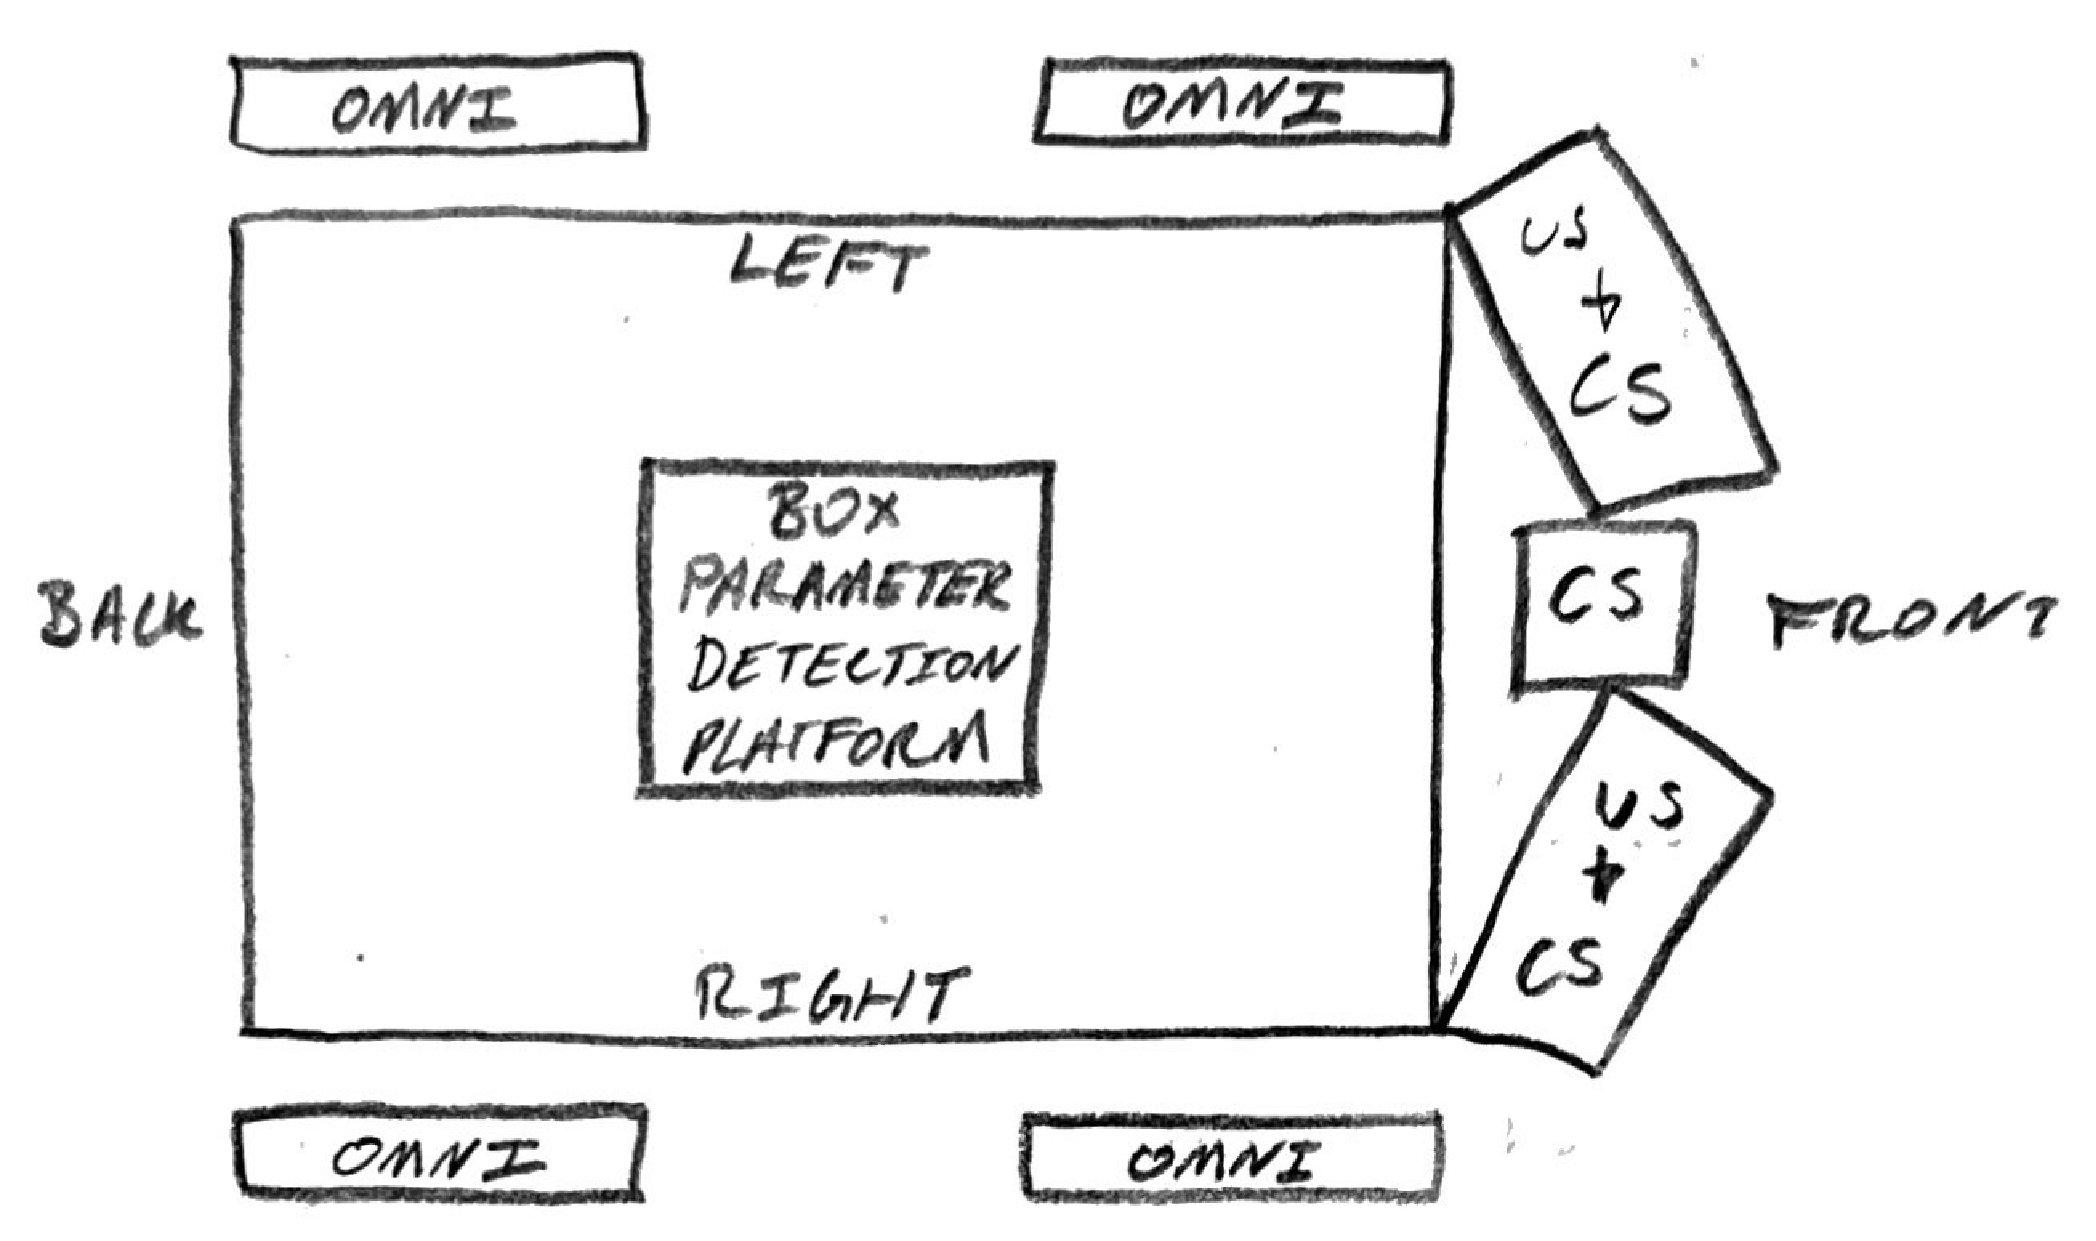
\includegraphics[width=0.5\linewidth]{Images//Designs/Design2a.pdf}
    \caption{Design2a - simplified layout of movement and sensor systems}
    \label{fig:design2a}
\end{figure}
The second design functions nearly identically to \cref{sec:design1} but with minor alterations to the sensor layout, as well as the introduction of \gls{omni}-wheels.

\begin{description}
    \item[Wheel Configuration --] This design still utilizes a standard 2x2 wheel configuration, but instead utilizes \gls{omni}-wheels with 2 \gls{DoF}. The implementation of \glspl{omni} fixes some of the aforementioned problems with dynamicism by enabling the robot to pivot more easily and with more control.
    %
    \item[Sensor Configuration --] This iteration uses a similar sensor layout to the previous, but this time the ultrasonic sensors are angled outward slightly, in theory, reducing the time it takes to identify objectives, subsequently increasing the overall efficiency of the system. Additionally, a third color sensor is attached to the center of the robot to increase the available information during line following functions.
\end{description}

\begin{figure}[H]
    \centering
    \hspace*{6em}
    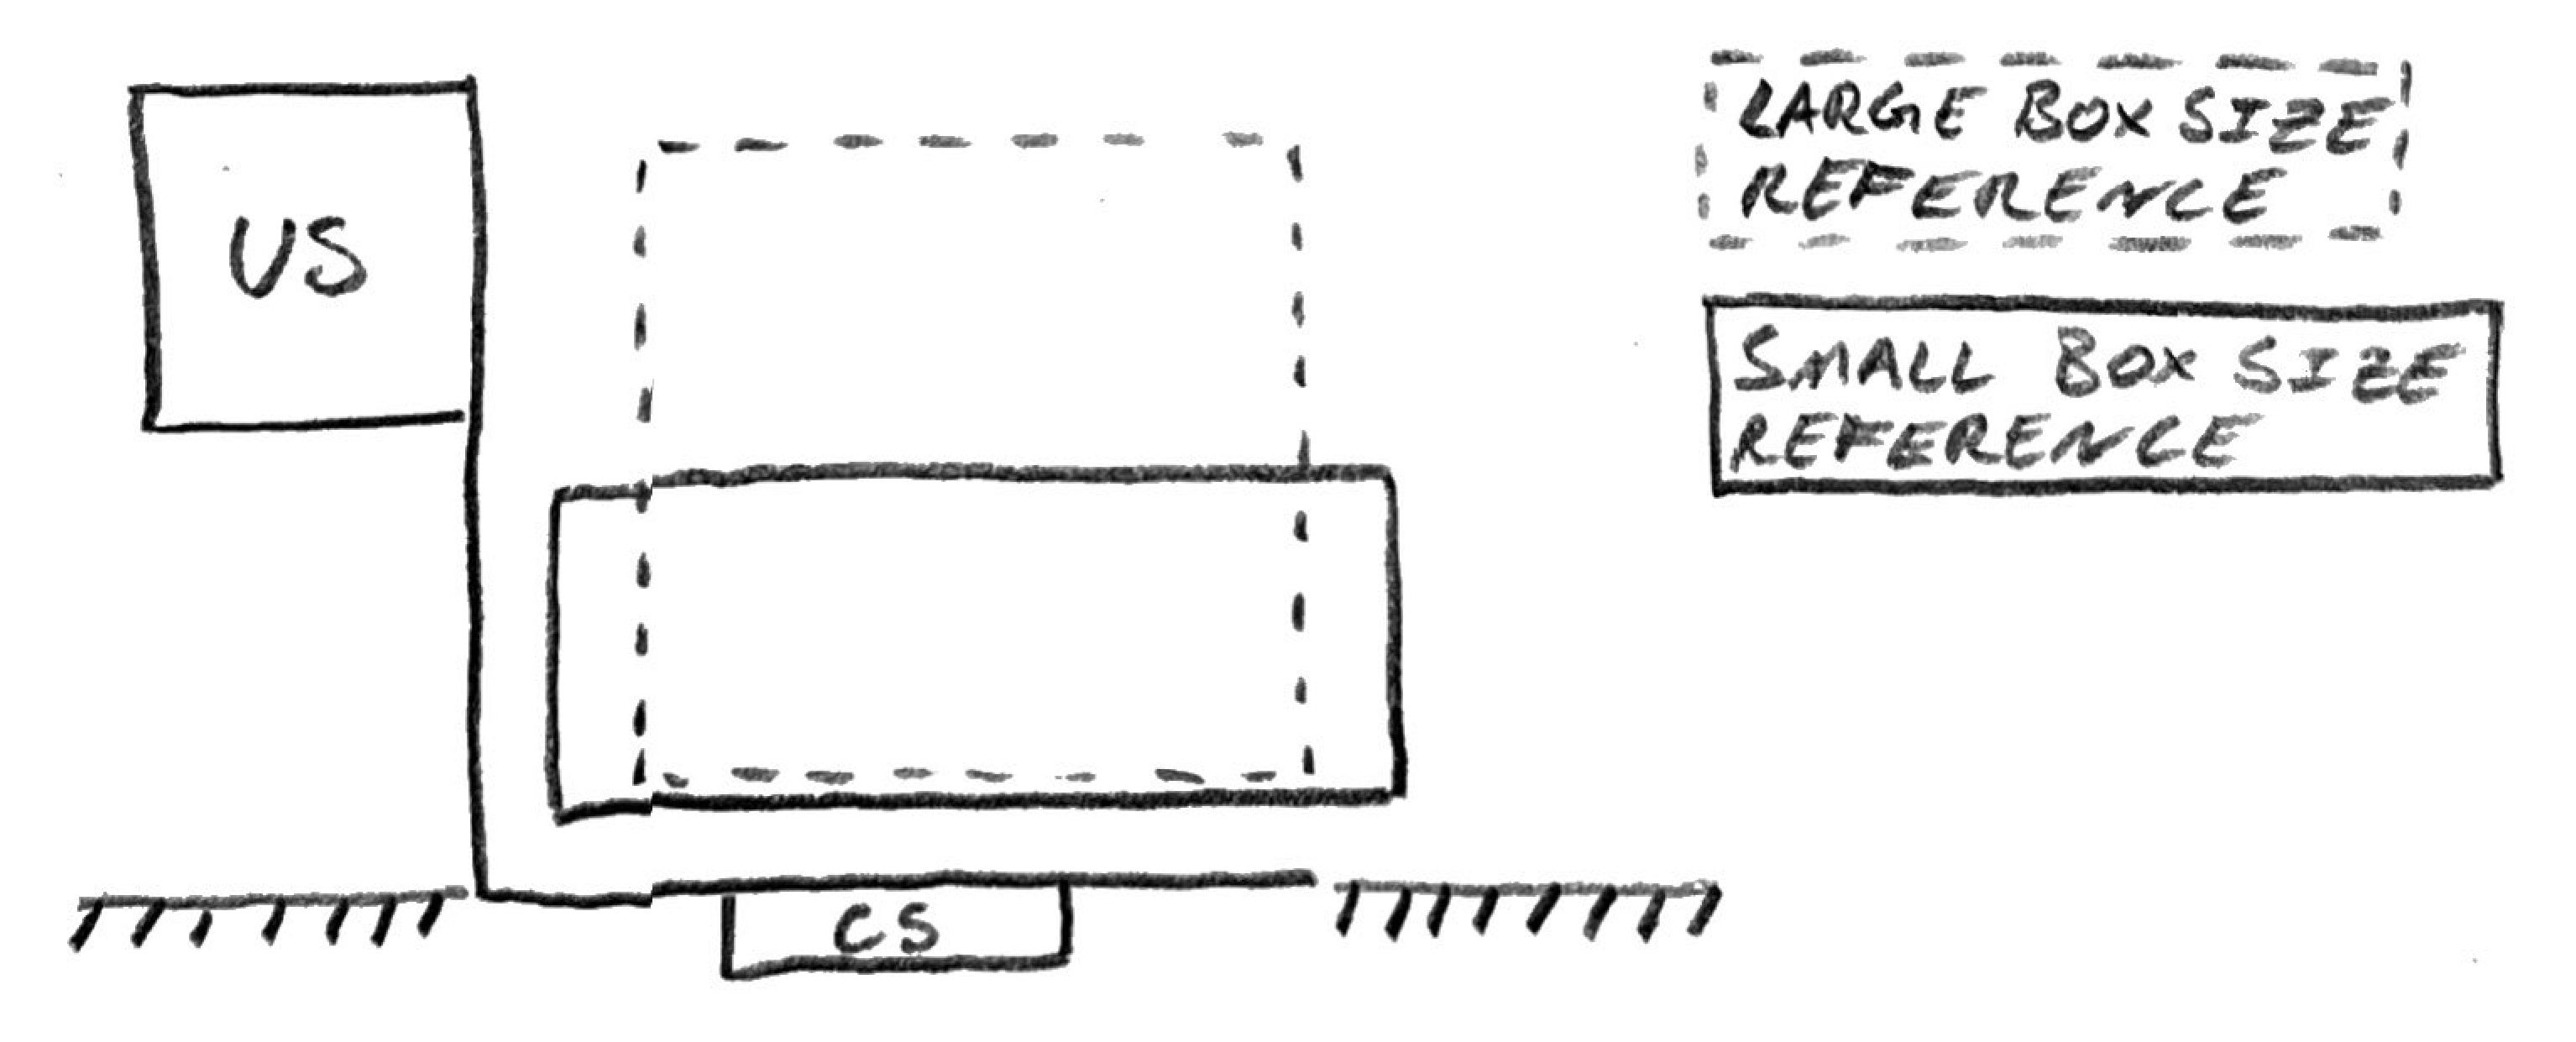
\includegraphics[width=0.6\linewidth]{Images//Designs/Design2b.pdf}
    \caption{Design 2b - Box property detection platform with \gls{IRS}}
    \label{fig:design2b}
\end{figure}
\begin{description}
    \item[Box Property Detection --]Again, a gripper mechanism places the box onto a platform that will then determine the properties of the package. An \gls{RGB} sensor is still used to get the color of the box, but an ultrasonic sensor replaces the \gls{IR} sensor. It should be noted that the swap from \gls{IRS} to \gls{US} was simply to provide another option during testing and assembly; there is no immediately identifiable benefit to using one over the other.
\end{description}

\newpage
\section{Design 3}\label{sec:design3}
\begin{figure}[H]
    \centering
    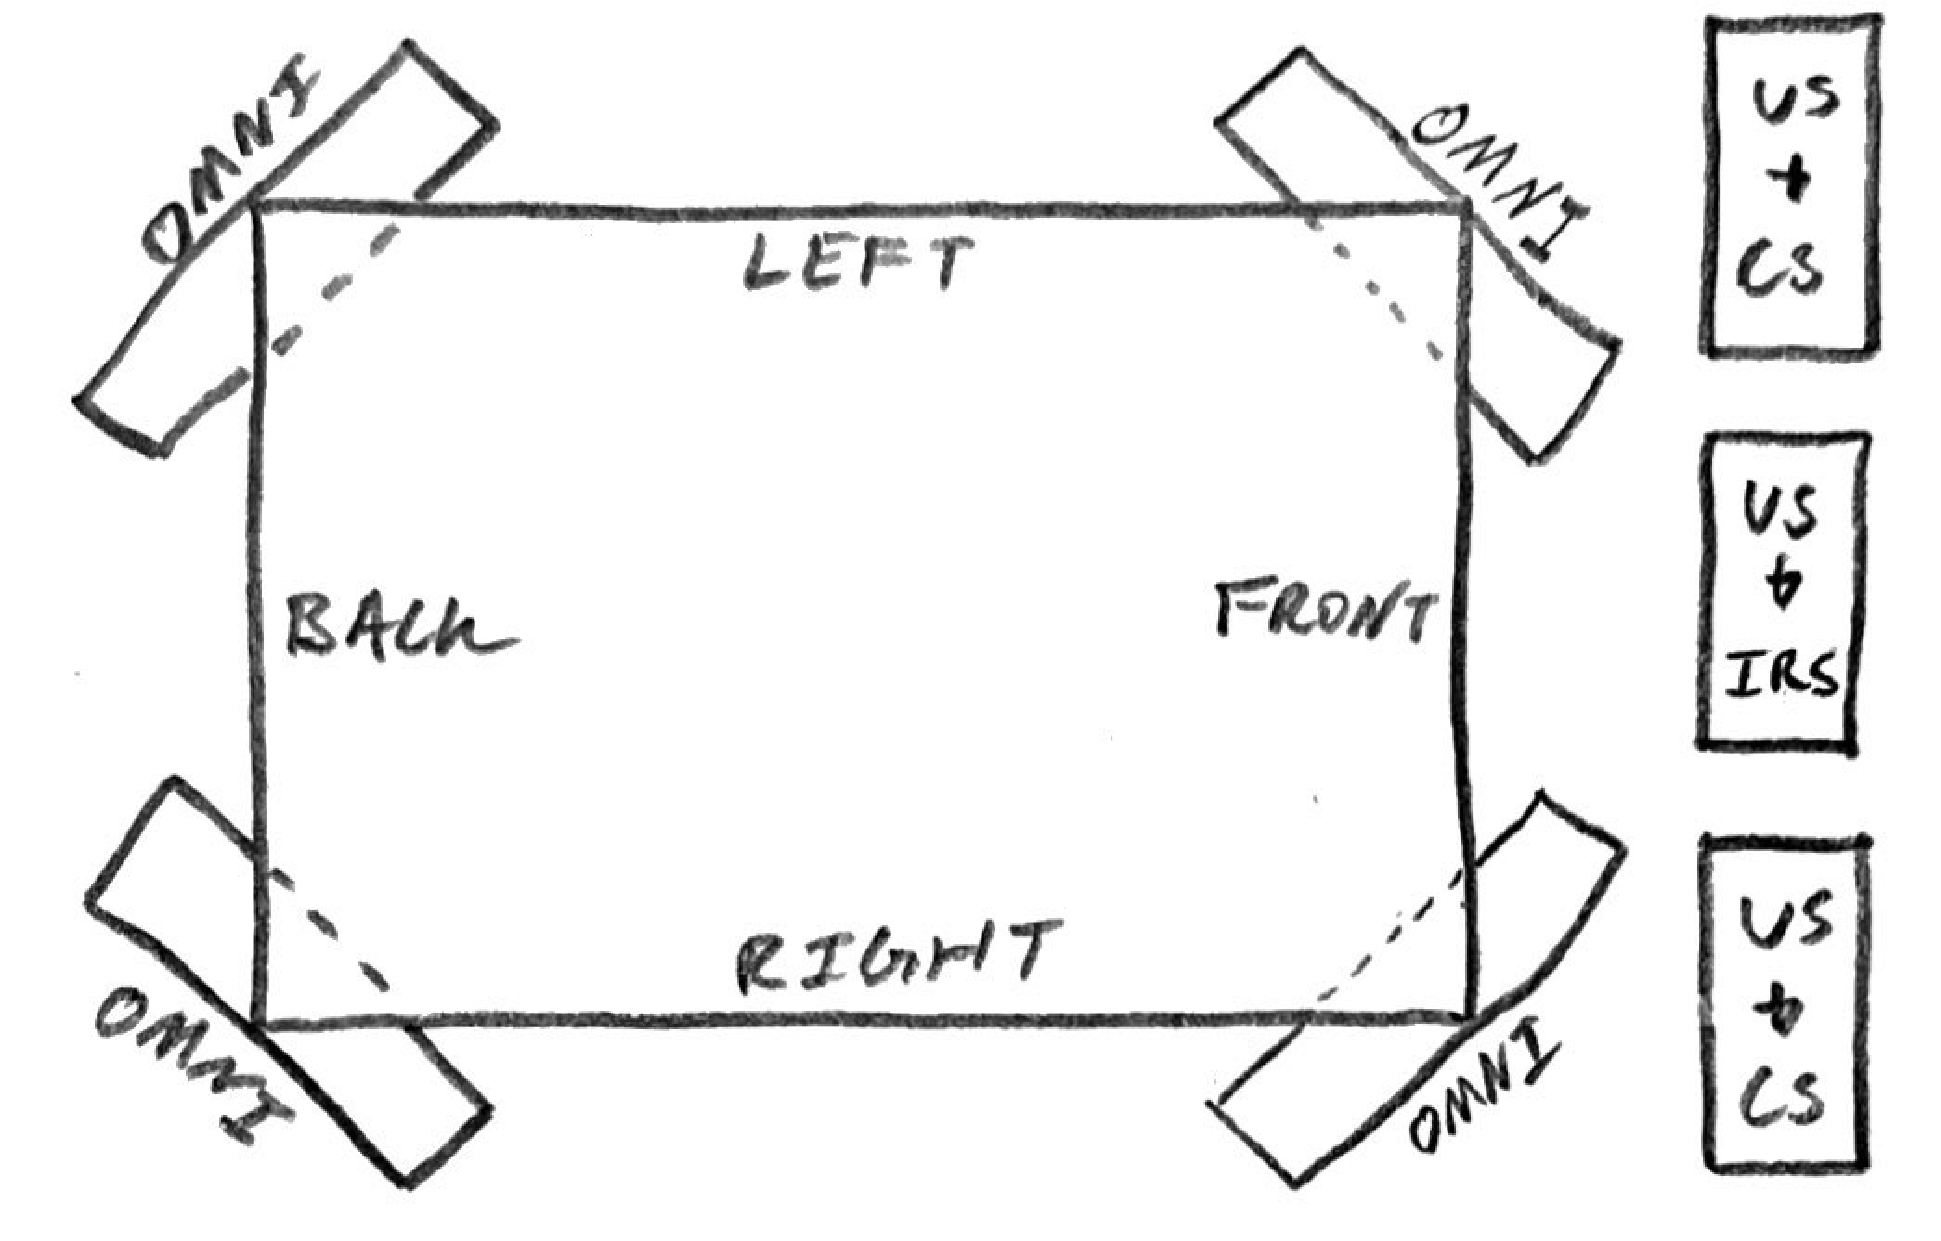
\includegraphics[width=0.5\linewidth]{Images//Designs/Design3a.pdf}
    \caption{Design 3a - simplified layout of movement and sensor systems}
    \label{fig:design3a}
\end{figure}
The third design introduces a new movement strategy, and features a new sensor layout intended for smarter movement capabilities.
\begin{description}
    \item[Wheel Configuration - ]The \glspl{omni} are now placed in a cornered configuration to enable crab-walking: linear translation in cardinal directions, or otherwise, via relative \gls{PWM} control.
    \item[Sensor Configuration - ]The ultrasonic sensors on the sides have been reverted to the original forward-facing orientation due to the addition of a third ultrasonic sensor. The side ultrasonic sensors are intended to be in-line with the wheels to predict possible collisions across the whole robot, and the centrally located one allows for faster targeting of the pick-up-and-place platforms. Lastly, two or more centered \gls{IR} sensors are utilized for line-following purposes.
\end{description}
\begin{figure}[H]
    \centering
    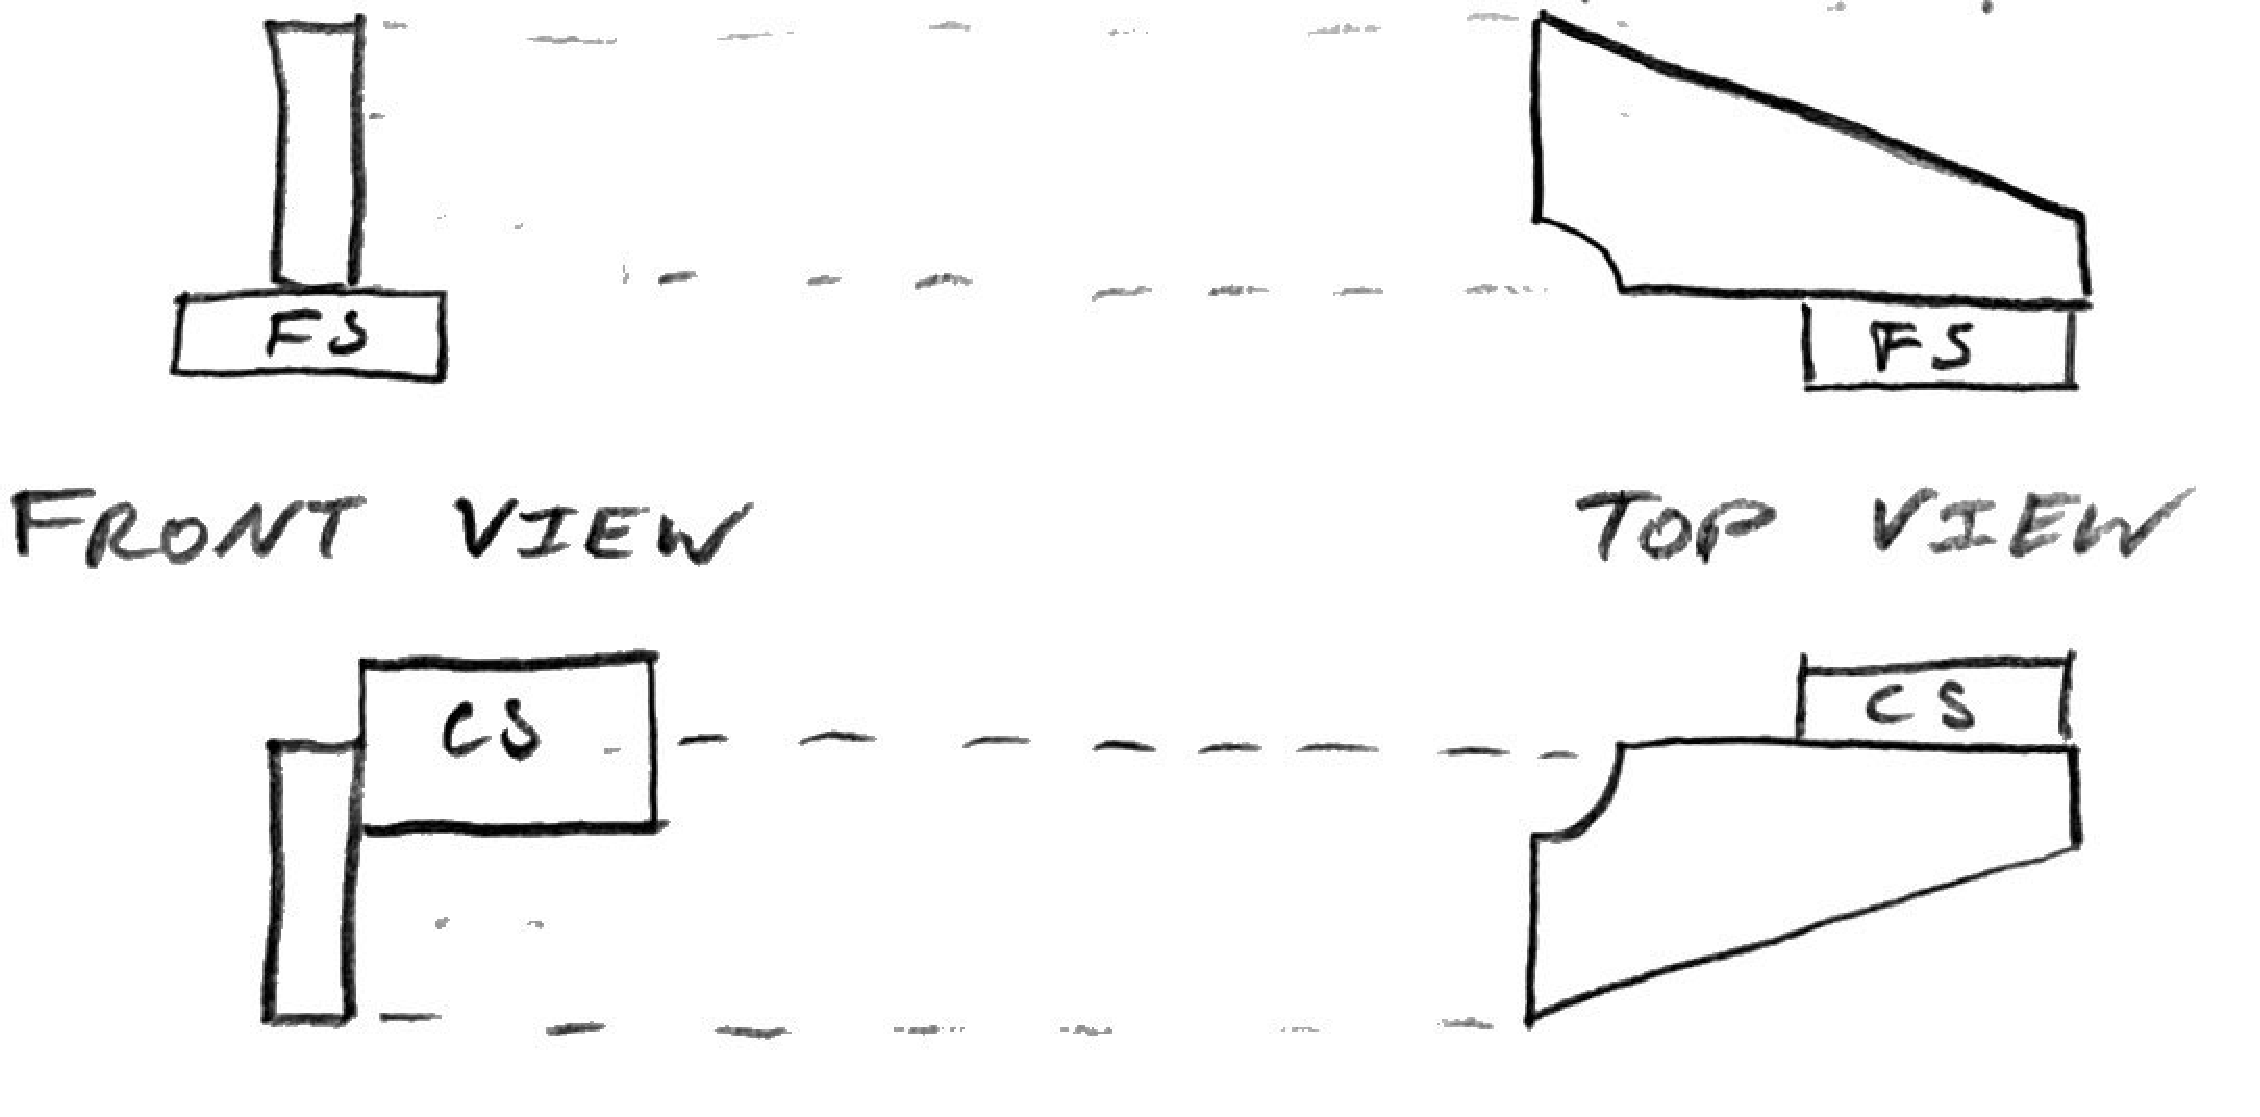
\includegraphics[width=0.5\linewidth]{Images//Designs/Design3b.pdf}
    \caption{Design 3b - Box property detection platform with \gls{IRS}}
    \label{fig:design3b}
\end{figure}
\begin{description}
    \item[Box Property Detection - ]This iteration removes the property detection platform entirely and includes all relevant sensors on the gripper itself via 3D printed mounts. The color sensor will be mounted on one mandible, while a force-sensor, denoted \gls{FS}, using a timing-based algorithm to determine box size will be placed on the other.
\end{description}

\newpage
\section{Design 4}\label{sec:design4}
\begin{figure}[H]
    \centering
    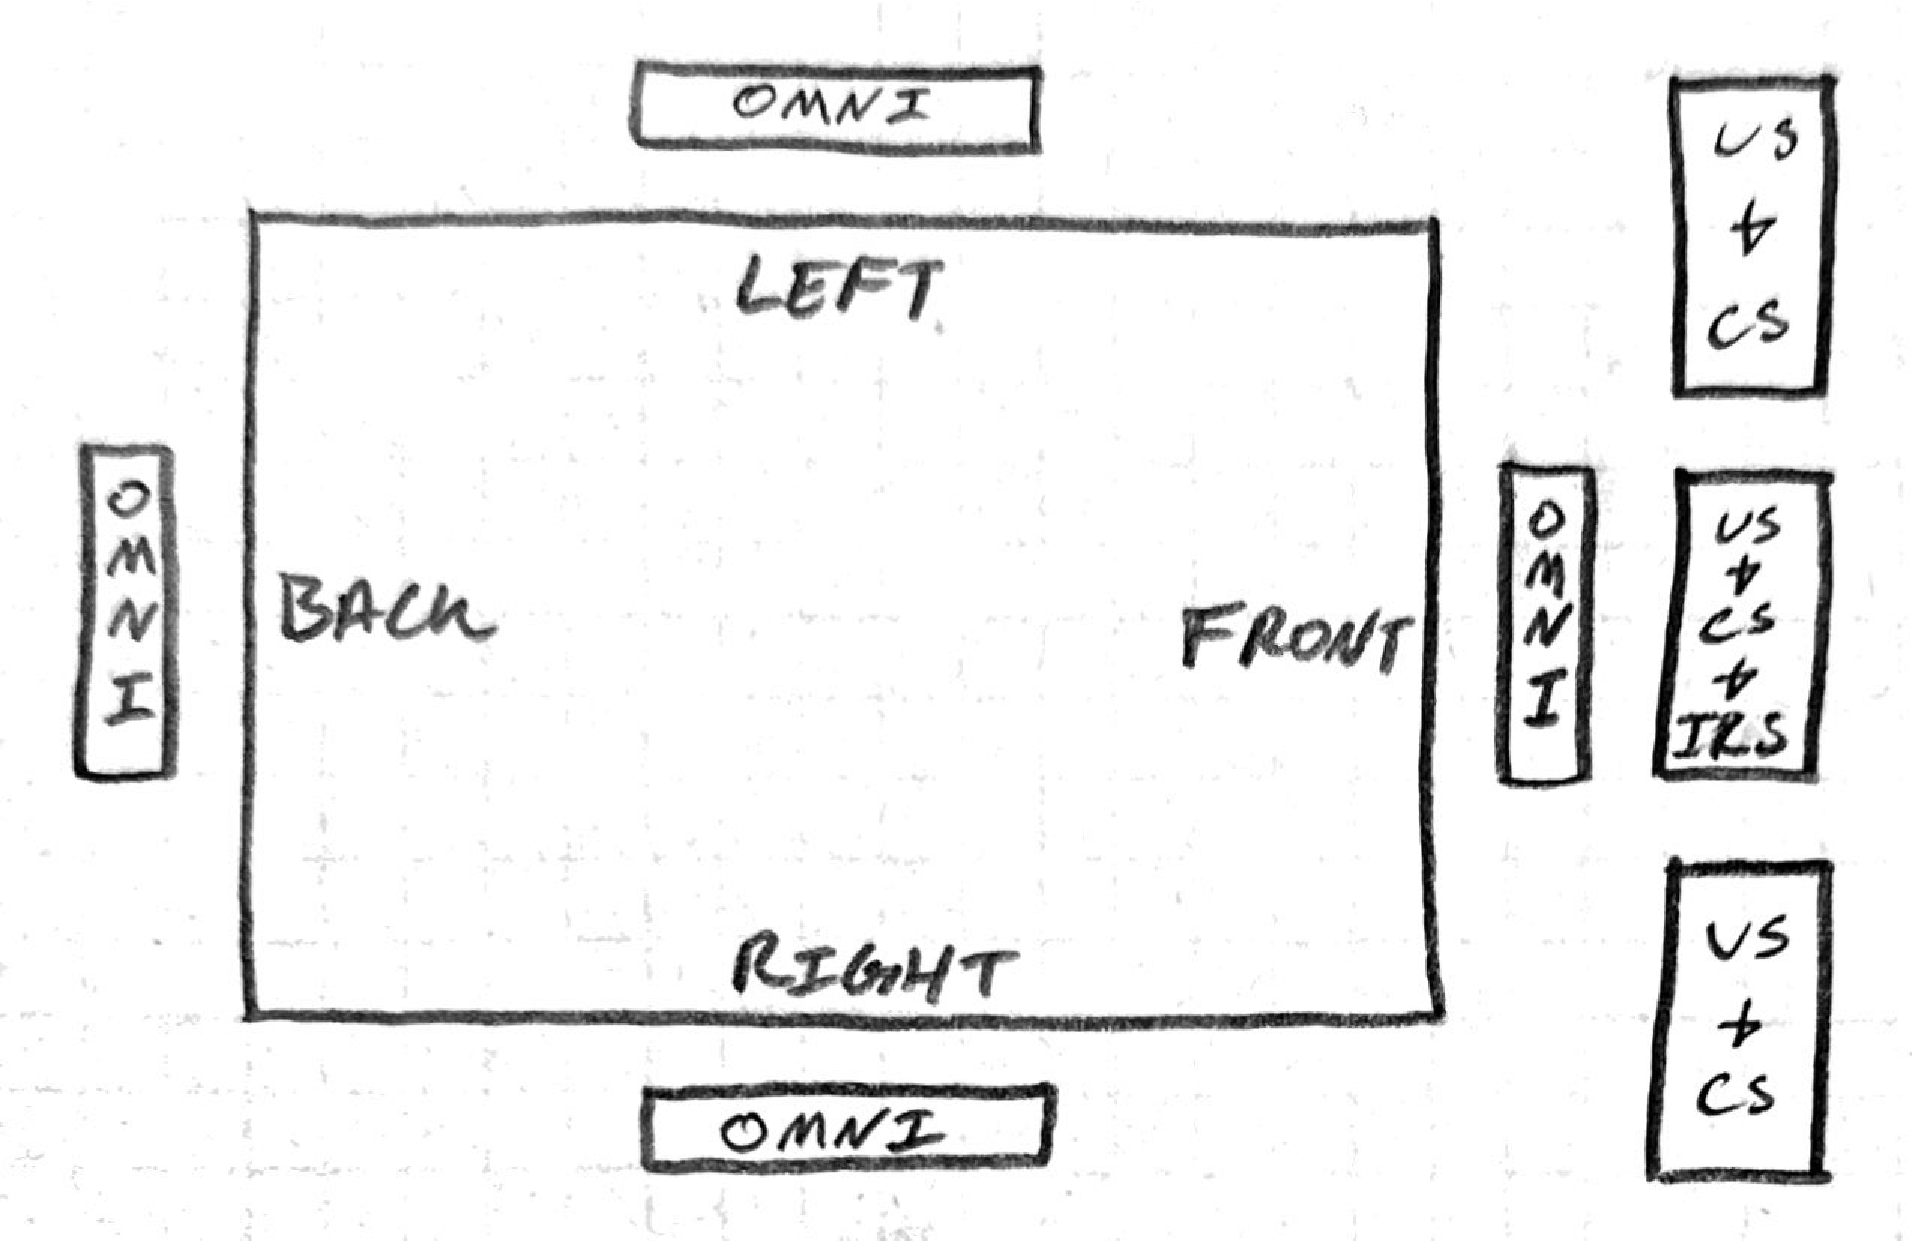
\includegraphics[width=0.5\linewidth]{Images//Designs/Design4a.pdf}
    \caption{Design 4a - simplified layout of movement and sensor systems}
    \label{fig:design4a}
\end{figure}
The fourth design reorients the wheels as to be square against the sides, and combines the ideas for centralized sensors of \cref{sec:design2} and \cref{sec:design3}. This was chosen as the final design; the decision matrix supporting this design ca
\begin{description}
    \item[Wheel Configuration - ]The \glspl{omni} are now placed in a squared configuration to increase the maximum speed potential, as the cornered configuration has inherent losses in the cardinal directions --- those most relevant to the tasks presented.
    \item[Sensor Configuration - ]This iteration uses the middle color sensor idea from \cref{sec:design2}, and the centralized \gls{IR} array and ultrasonic sensor from \cref{sec:design3}. Together, these sensors provide as much information about the robot's location and orientation as possible.
\end{description}
\begin{figure}[H]
    \centering
    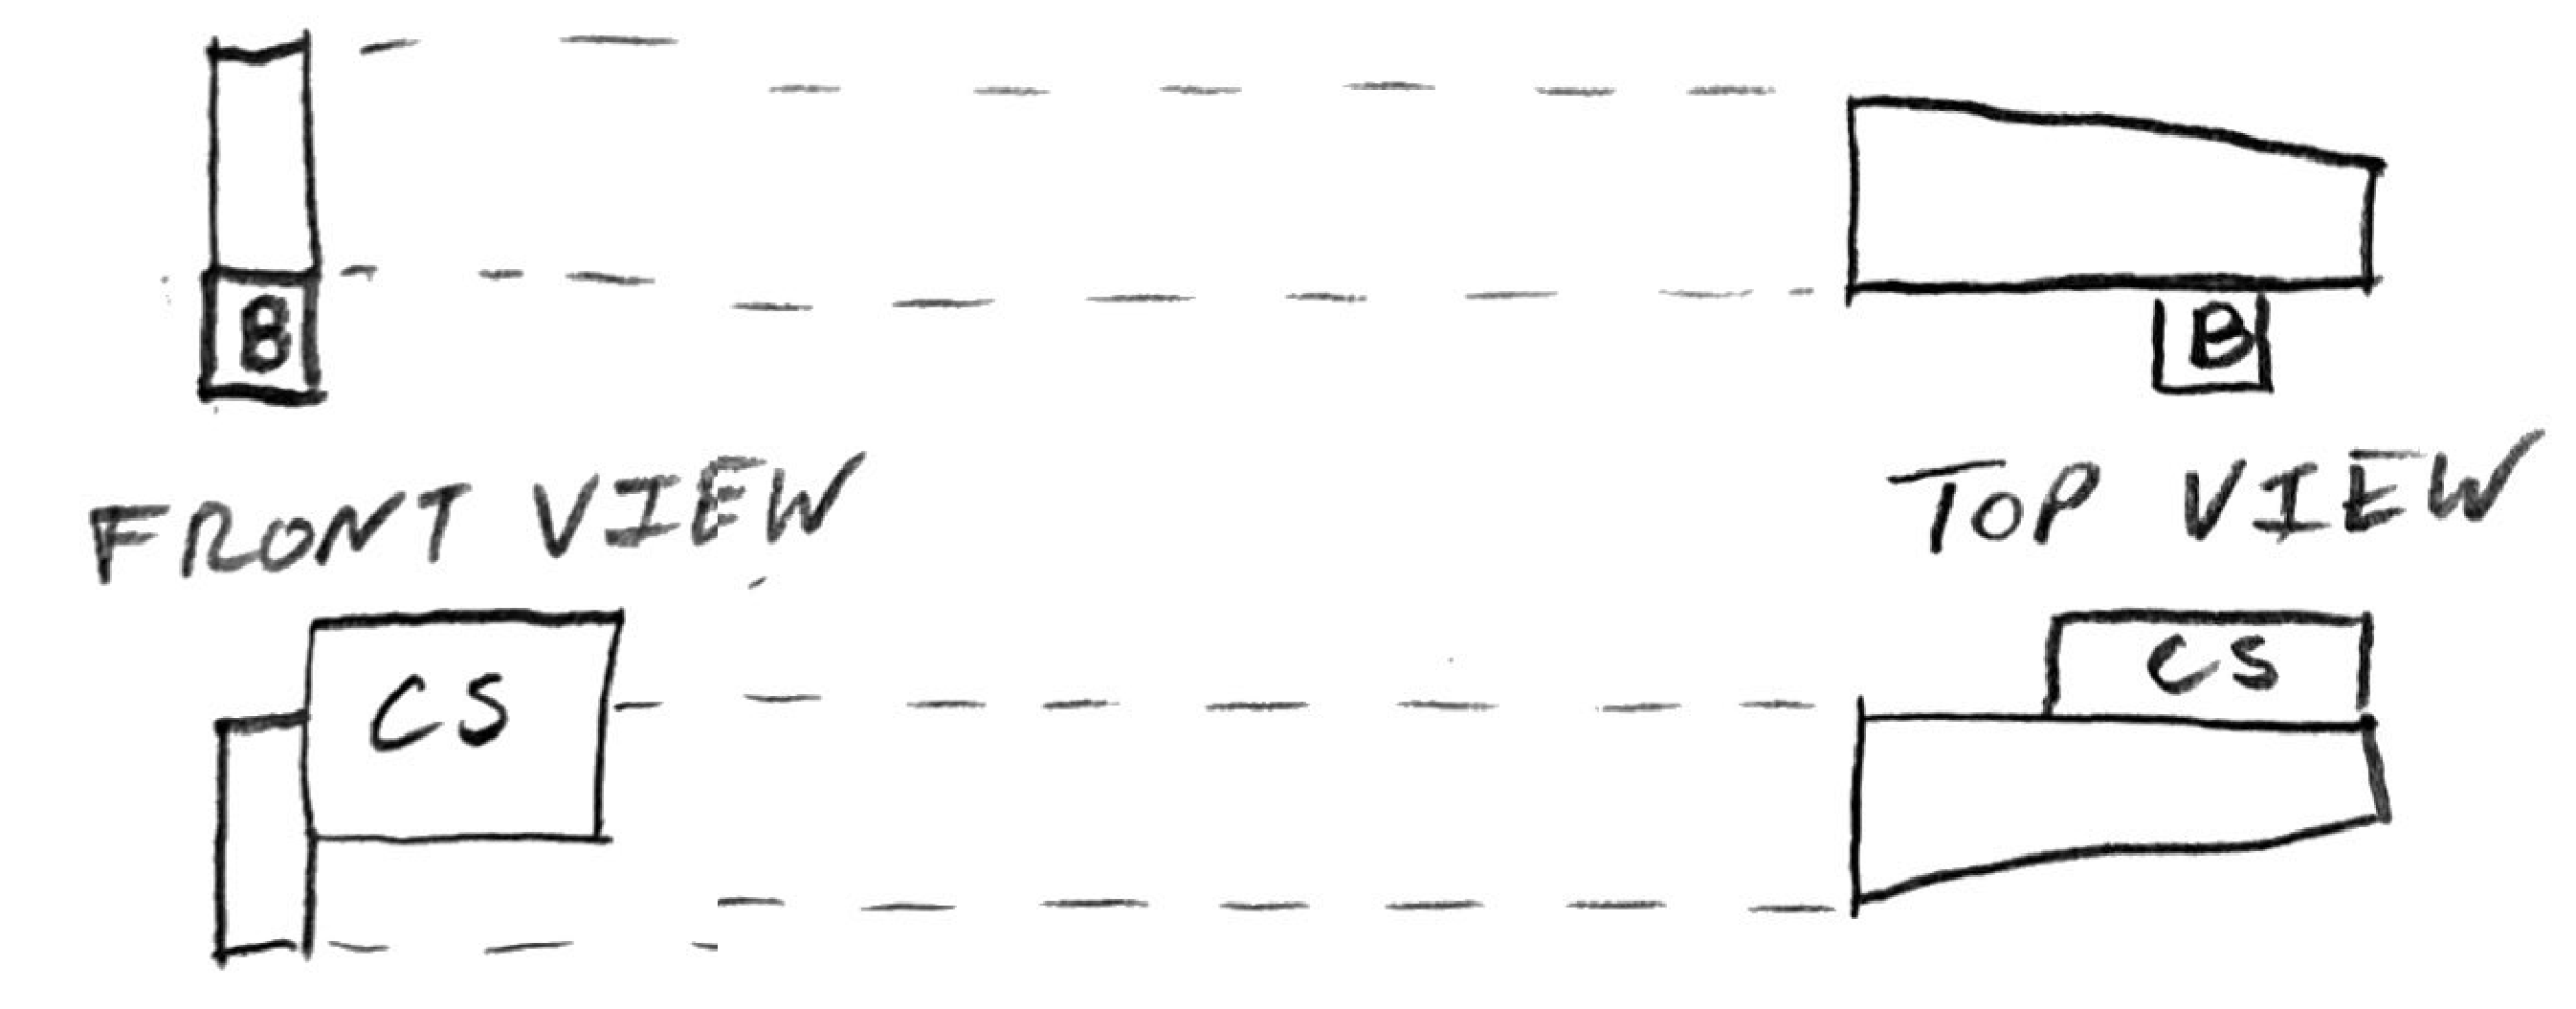
\includegraphics[width=0.5\linewidth]{Images//Designs/Design4b.pdf}
    \caption{Design 4b - Box property detection platform with \gls{IRS}}
    \label{fig:design4b}
\end{figure}
\begin{description}
    \item[Box Property Detection - ]This gripper sensor layout is identical to the last with a button, denoted \gls{B}, in place of the force sensor, which will operate under a similar algorithm while eliminating the inconsistency of the force sensor.
\end{description}

\end{document}
\documentclass[11pt]{report}
\usepackage{StyleSheets/main}
\begin{document}

\chapter{System Risk Management}\label{ch:system-risk-management}
The purpose of this section is to manage the possible risks of this system. Possible risks will be identified, and solutions for risk mitigation will be brought forward. This section is an important way for the team to be prepared for any possible setbacks and to limit the amount of setbacks taken in an effort for the project to run smoothly.

\begin{figure}[H]
    \centering
    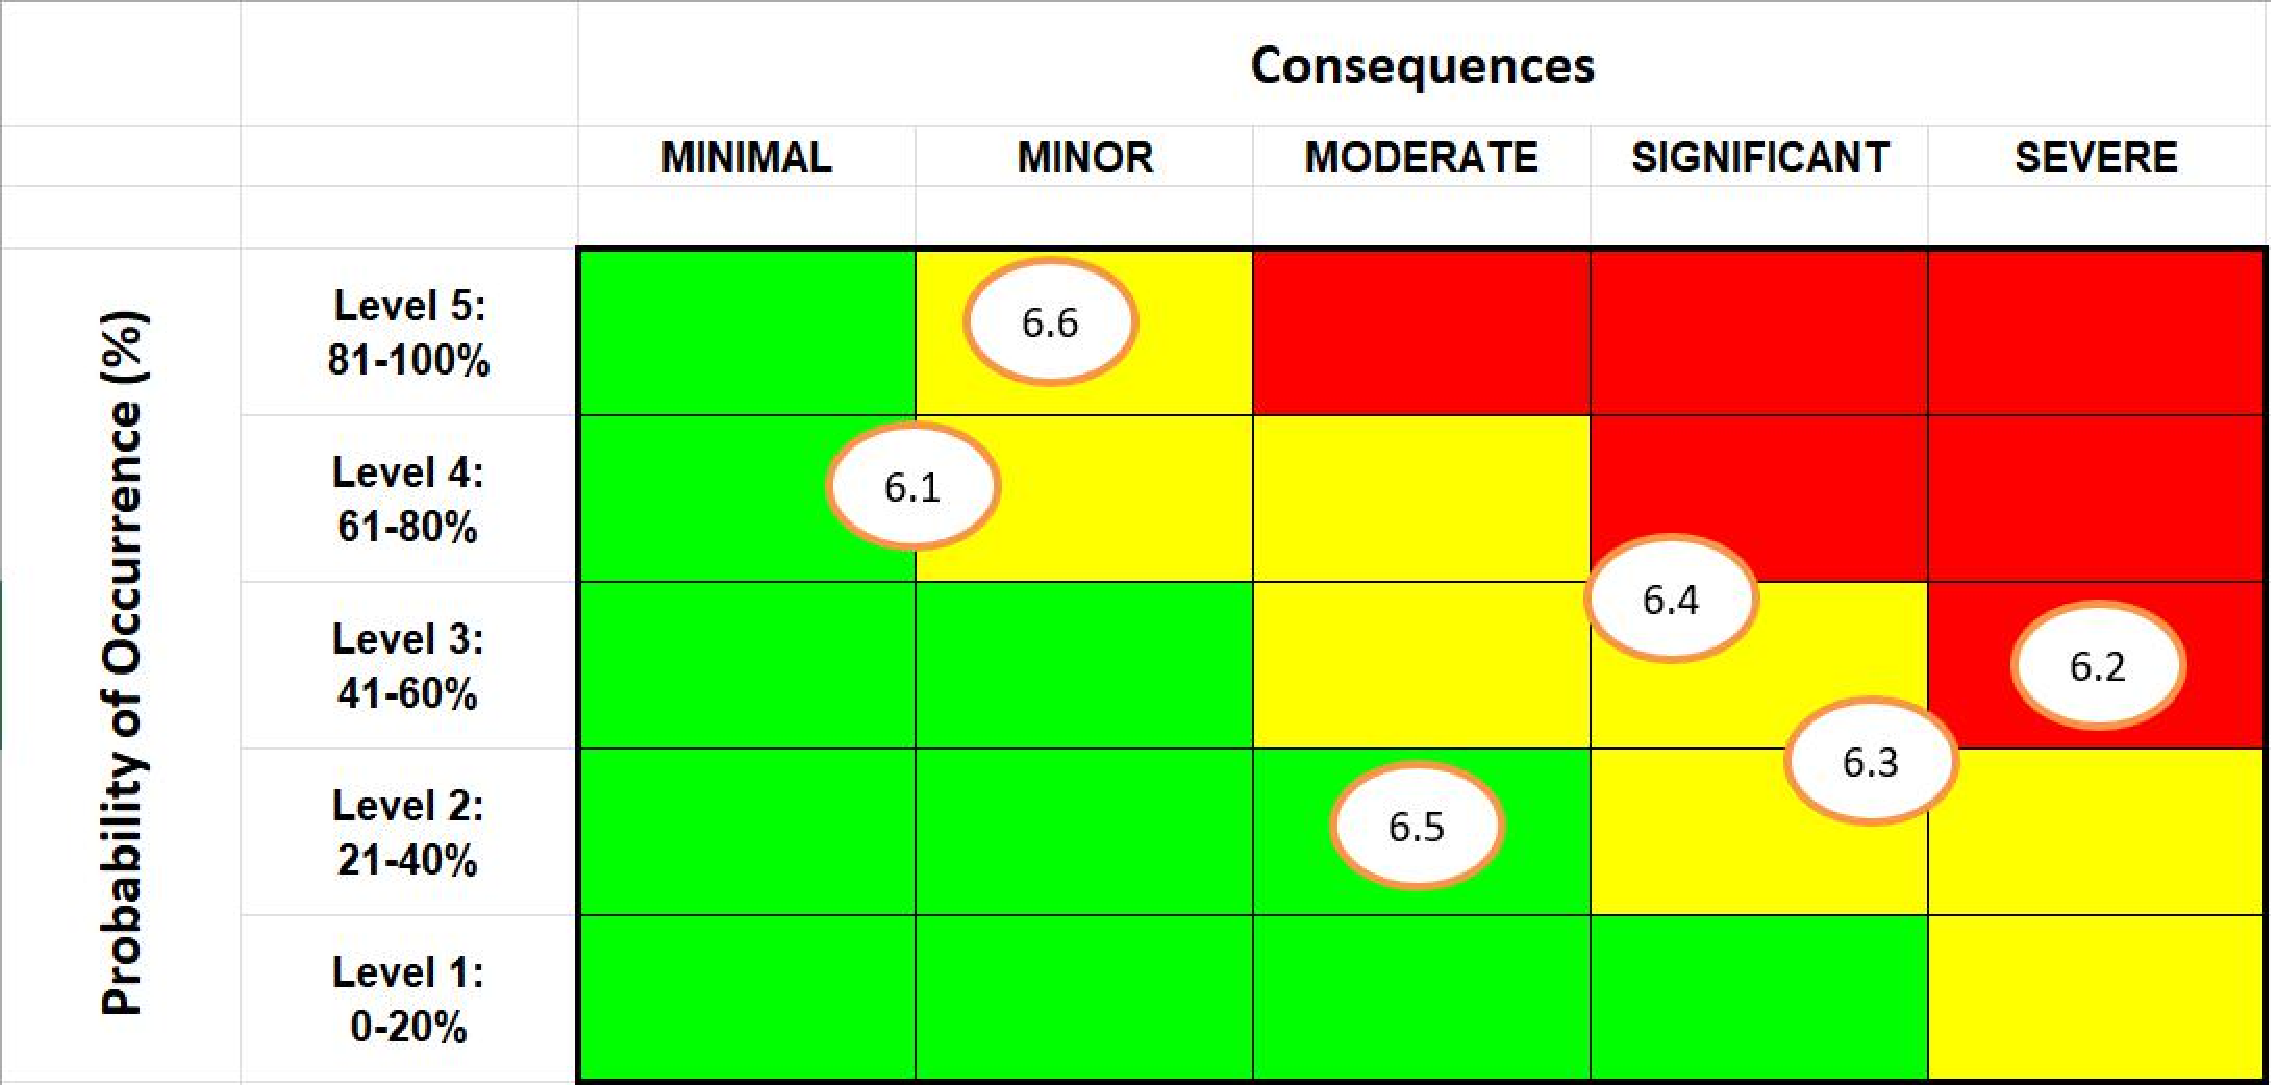
\includegraphics[width=0.8\linewidth]{Graphs/SystemRiskManagementGraph.pdf}
    \caption{System Risk Management Assessment Graph}
    \label{fig:system-management}
\end{figure}

\section{Failure of 3D Prints during printing}
\begin{itemize}
    \item Risk: This system required a lot of 3D prints for sensor mounts and vehicle structure. It is possible that during printing these prints fail due to the nature of 3D printing. 
    \item Mitigation: If multiple of the same print are printed at a time, the risk of a print failing is greatly reduced. Introducing redundancy into 3D prints is a great way to lose the uncertainty of a print failing. For example, if a sensor mount has enough space on the printing board for 2 or even 3 prints, the maximum amount of prints should be done just in case of the event of failure. 
\end{itemize}
\section{Burning of an Electrical Feature}
\begin{itemize}
    \item Risk: During robot testing, it is possible for a wire to be misplaced or a mistake to be made resulting in an electrical feature in the robot heating up, burning, and possible becoming permanently damaged. Electrical features in this system which are at risk of this issue are the Teensy microcontroller, the motor controllers, and the \gls{DC}--\gls{DC} converters. This can also become a risk to the user of the vehicle, as it could result in an electrical fire or the user getting hurt or injured.
    \item Mitigation: In the event of an electrical part burning, a new part can be bought, however it is better for this not to be the case. When handling voltages which are capable of destroying sensitive parts, care must be taken to avoid the damage of these parts. 
\end{itemize}
\section{Failure or Breaking of a Motor} 
\begin{itemize}
    \item Risk: During testing of the robot, it is possible that a motor becomes incorrectly placed or incorrectly wired. This can result in damage to the motor, which is a massive risk to the system
    \item Mitigation: While a new motor can be bought for the system, it is better to avoid this as it is out of budget. When handling the motor, it is essential that the motor is handled and installed with care. 
\end{itemize}
\section{Damage to Parts During Soldering}
\begin{itemize}
    \item Risk: During soldering of parts of the vehicle, it is possible that the soldering iron can burn parts of the robot. The temperatures which are being dealt with during soldering are very high and would break any part which is made contact with. 
    \item Mitigation: During soldering of wires and parts, extreme care must be taken to not damage the parts of the vehicle. Care must be taken to ensure that the soldering iron does not come in contact with the motor or other easily damaged electrical parts of the vehicle.
\end{itemize}
\section{Running out of Budget for the System}
\begin{itemize}
    \item Risk: It is a risk that the budget for the system is exceeded. This can limit the changes which are made to the vehicle due to the lack of funds available. 
    \item Mitigation: Cost saving measures should be taken throughout the project. Attempting to save as much money from the budget as possible is essential, while care must be taken to not cut corners and induce other failures in the system from this. 
\end{itemize}
\section{Lack of Correspondence of Color Sensors}
\begin{itemize}
    \item Risk: With past experience and knowledge of the color sensors used in this system, it is known that the color sensors are very difficult to work with and are very sensitive to external light or shiny surfaces.
    \item Mitigation: It is important to not let the color sensors be affected by external light. This can be done by introducing ``curtains'' around the color sensors to ensure that the only light which is seen by them is their own light. Reducing the amount of variables around the color sensors is important in ensuring their accuracy. It is also important to calibrate the colors and surfaces on which the vehicle will be running to reduce the sensitivity of the system to shiny or reflective surfaces. 
\end{itemize}
\end{document}

\documentclass[11pt]{report}
\usepackage{StyleSheets/main}
\begin{document}

\chapter{Detailed Design}\label{ch:detailed-design}
This section will give a detailed design of the vehicle, its components, and special design features. It is to serve as a breakdown of the vehicle's structure, detailing every part of the vehicle. In this section, the vehicle's special design features, a decomposition of the structure, circuitry of the vehicle, and the software architecture will be discussed and detailed. 

\section{Body of the Vehicle}

\subsection{General Structure}
The base of this vehicle's structure is a singular 1116 Series Grid Plate (to be referred to as bottom grid plate). This grid plate has a  17 x 29 hole configuration, with each hole being $\SI{4}{\milli\meter}$ in diameter. The size of the bottom grid plate is 136 x $\SI{232}{\milli\meter}$, and is $\SI{2.5}{\milli\meter}$ thick. This grid plate serves as a strong and sturdy base for the structure of the vehicle, and is at the core of all connections made. One of the ends of this bottom grid plate will be referred to as the front, which mounts the ultrasonic sensors, gripper, and color sensors. At the back end of the vehicle were 2 U-shaped connecting pieces, which served as a cover for the battery. These U-shaped pieces were placed on both sides of the vehicle, and the $\SI{12}{\volt}$ battery was placed with its full length being perpendicular to the length of the grid plate. On top of this U-shaped connector, was placed another grid plate. This grid plate was of the same specification as the original grid plate, although it was also placed perpendicular to the length of the bottom grid plate, and in the same orientation as the battery. Two breadboards were placed on this top grid plate. One breadboard served as a place to house the Teensy 4.1 microcontroller, and the other was used for power distribution around the circuit as well as an \gls{LED} to indicate the state of the system. The breadboards and Teensy 4.1 microcontrollers are discussed in \cref{sec:wiring,sec:breadboard-and-pins}.

\par The gripper was placed on the front of the bottom grid plate. The structure of the gripper is discussed in \cref{sec:gripper}. On either side of the gripper a mount was placed for the ultrasonic and color sensors. These sensor mounts allowed for the vehicle to complete the tasks of color recognition, obstacle avoidance, and line following. Underneath the bottom grid plate sat the motor controllers which were placed with spacers between the plate and the controllers to avoid unwanted interruptions in the circuit. 2 motor controllers were used, each powering 2 of the 4 motors used. The 4 motors, attached to the vehicle using 2 side clamping mounts, were placed on each side of the vehicle, in the middle of each length. These mounts were placed underneath the bottom grid plate, and each had a brushed \gls{DC} 26 \gls{RPM} motor attached. To the ends of these motors, was attached an omni wheel, which allowed the vehicle to move in any direction in a crab-walk configuration. Over the front wheel and underneath the gripper was placed a sensor mount, which allowed for the attachment of an additional ultrasonic sensor in front of the vehicle, which was in the center and further forward than the other sensors. 

\subsection{Wheels}
The system utilized a crab-walk design, having a wheel on either side of the vehicle as well as the front and back. This configuration allowed for the vehicle to have 2 degrees of freedom in movement, with the side wheels allowing for forward and backwards movement and the back and front wheels allowing for side to side movement. The wheels, which were chosen to be omni-wheels, allowed for the smooth movement of the vehicle in every direction. This design allowed for higher speeds in every direction, with each direction of movement allowing 2 motors to push the necessary wheels. 
\par During testing, the issue of the wheels slipping during sideways movement of the vehicle came up. The weight was unevenly distributed throughout the robot, causing it to not allow the side wheels to both be in contact with the ground at a time. The solution for this problem was to introduce a suspension system, which allowed the motor mounts to bend outwards allowing the vehicle to have all wheels in contact. On the right side of the vehicle, a spring was placed along with a series of washers to the motor mounts connection points with the grid plate. This allowed the connection to be looser and have more flexibility. On the other side of the vehicle, the bottom of the motor mount included springs, which pulled the wheel closer to the vehicle but allowed for more flexibility. The introduction of the suspension system allowed the robot to move in every direction effectively. 

\subsection{Motors}
The motors attached to these wheels were 26 \gls{RPM} \gls{DC} motors. These motors provided the vehicle with the necessary speed to complete the tasks in a faster time. The side 26 \gls{RPM} motors were modified using 116 \gls{RPM} motor’s gearboxes, which gave the vehicle additional speed in the forward and backward directions. 

\subsection{Battery}
The battery used in this vehicle was a $\SI{12}{\volt}$ battery with an on and off switch, a charging port, and a connection port for wires to be connected to the rest of the circuit. All of the vehicle’s power came from this battery. The placement of the battery allowed for easy changing between on and off during testing, which simplified the process massively. The battery being situated at the back of the vehicle allowed for the weight to be distributed evenly throughout the vehicle, as it balanced the weight of the gripper on the front. The wiring of the battery to the rest of the circuit will be discussed in later sections. 

\subsection{3-D Printed sensor mounts}
\subsubsection{Ultrasonic Sensor and Color Sensor Mounts}
The ultrasonic sensors and color sensors were placed on the 3D printed sensor mounts. The design is shown in Figure B.12. These mounts were attached to the bottom grid plate on either side of the vehicle’s front wheel. The side sensor mounts were designed to house the ultrasonic sensors in a position where they would sense further outwards than the furthest edge of the wheel to avoid the vehicle hitting the obstacles during the tests. The ultrasonic sensors were placed in a forward facing position, while the color sensors were attached facing towards the floor for color recognition. The color sensors were housed by a curtain as a part of the sensor mounts to avoid external light messing with the color sensing ability.
\subsubsection{Front-Central Ultrasonic Sensor Mount}
The middle ultrasonic sensor mount had a design to which it would attach to the top of the bottom grid plate and curve over the top of the front wheel. This curve was such that it would not interfere with the front wheel, and there was sufficient space for the attachment of wires to the ultrasonic sensor without interference. This design allowed for the central front facing ultrasonic sensor to be further forward than the rest of the vehicle, and allowed for the vehicle to sense the platform on which the box is located for the pickup and placement test. The front-central ultrasonic sensor mount can be seen in Figure B.8.

\subsubsection{Lower Infrared Sensor and Color Sensor Mount}
The vehicle’s \gls{IR}/\gls{RGB} sensor mount was located beneath the vehicle, and allowed for the sensors to be as close to the ground as possible for accurate centering about the target-line. The mount was attached to the motor mount of the front wheel, and the \gls{IR} sensor was located right underneath this mount. The sensor mount also acted as an electrical spacer to avoid unwanted contact with metals and the \gls{IR} sensor. The lower \gls{IR} sensor mount can be seen in Figure B.9. 

\section{Gripper}\label{sec:gripper}
\subsection{Gripper Arm}
The arm of the gripper was made up of many plates and connecting pieces. Firstly, a U-shaped connection plate was attached to the front of the vehicle, occupying the same holes in the grid plate as the front-central ultrasonic sensor and the front wheel. This U-shaped plate raised the gripper above the vehicle and allowed for the gripper to not come in contact with the wheel. Attached to this is another U-shaped plate of the same shape, and inside this is the servo motor which controls the movement of the gripper arm. This servo motor allows the gripper to move with one degree of freedom, and controls the angle at which the gripper is facing. The servo motor is attached to the rest of the arm using a metal rod which is attached to a longer plate. This longer plate extends the length of the gripper arm, and allows the hand of the gripper to reach the box in the pickup and placement system. The end of this arm plate marks the end of the gripper arm before the hand system starts, with a U-shaped grid plate attached to the end of the arm. 
\subsection{Gripper Hand}
The gripper hand is made up from multiple smaller components. Attached to the gripper arm is the claws of the gripper, which are 2 pieces of plastic with extensions to reach the box. These extensions are controlled using a gear system which is connected to another servo motor, which has the use of controlling the opening and closing of the gripper hand. The ends of the extensions have 3D printed mounts attached, which will be detailed shortly. 
\subsection{Gripper Sensor Mounts and Sensors}
The sensors for the gripper hand were attached to the claw of the gripper using 3D printed sensor mounts. The sensors on the gripper were used to determine box size, box color, and height of the gripper above the platform. 
\subsubsection{Left Gripper Sensor Mount and Sensors}
The left sensor mount was used as an extension to the gripper claw which allowed for the vehicle to more effectively grab the box. Within the extension was placed the color sensor, which had the task of sensing whether the box was blue or red. The left gripper sensor mount can be seen in Figure B.11.
\subsubsection{Right Gripper Sensor Mount and Sensors}
The sensor mount on the right hand side of the vehicle’s gripper had the purpose of allowing the box to be better grabbed as it was an extension of the claw, and also served as a place for an infrared sensor and a button. The infrared sensor allowed the robot to know when it was near the platform and could drop the box. The button had the purpose of letting the robot know which size box was being picked up. The time from when the gripper started closing and when the button was pressed was measured and the robot used this information to determine the box size. The right gripper sensor mount can be seen in Figure B.10.

\subsection{Added Component Cost}
A total of \$1.65 of the provided \$25 budget were used for both prototyping and final iterations of the aforementioned sensor mounts, and another \$4.99 for the \gls{IR} array. 3D-prints were done efficiently by sending multiple of the same design to print simultaneously to avoid failures that would further delay our design and testing processes. A complete breakdown of the cost, including both the 3D-printing and \gls{IR} array, can be found in \cref{ap:diagrams}.

\section{Breadboards and Pins}\label{sec:breadboard-and-pins}
\subsection{Teensy 4.1 Microcontroller}
Placed on one breadboard was the Teensy 4.1 Microcontroller. The microcontroller was an integral part of this system which allowed a computer to communicate with the robots movements and features using code which was implemented to the system. The Teensy 4.1 microcontroller has a series of pins which connect to the color sensors, the ultrasonic sensors, the infrared sensors, the motors (through the motor controllers), and the servo motors. The Teensy 4.1 pinout map can be seen in Figure B.14. 
\par Each pin in the Teensy 4.1 had a wire connecting it to the required part of the robot, in a complicated wire network which is discussed shortly. 

\subsection{DC-DC Converters}
The second breadboard used contained two \gls{DC}-\gls{DC} converters (buck converters). These were used to bring the voltage from the $\SI{12}{\volt}$ battery down to a more usable voltage for the system, and was controlled using a potentiometer built into the buck converter. 
\par One DC-DC converter was used to step down the $\SI{12}{\volt}$ from the battery to $\SI{7.4}{\volt}$ for the use of the motors which drive the vehicle. This voltage allowed the motors to operate at maximum capacity. The other converter was used to power the Teensy 4.1, stepping the voltage down to $\SI{5}{\volt}$.

\subsection{LED System}
The \gls{LED} system on the breadboard represented a system to show whether the battery was turned on or not. If the battery was on, the \gls{LED} would shine and if not, it would turn off. This helped know whether the system was active or not. The \gls{LED} was connected to the system using the voltage from the \gls{DC}-\gls{DC} converters and a resistor in series with the \gls{LED}.

\section{Wiring}\label{sec:wiring}
\subsection{Sensors}
In testing, it became clear that wiring would be an important factor for the simplicity of the system. The final robot had a simplified wiring system for the sensors. Each sensor has a set of pins to which connections need to be made. The color sensor pin map can be seen in Figure B.15. 
\par At the front of the robot, the sensor mounts allowed for the wires of the ultrasonic and color sensor wiring to be greatly simplified and to not interrupt any other use of the vehicle. The wires and wire extensions connected the sensors to the Teensy 4.1 microcontroller in their respective ports.

\subsection{Gripper}
The wiring on the gripper was important as it is a moving piece and could mess up the system if done incorrectly. The gripper, the servo motors, and the gripper sensors all connected back to the Teensy microcontroller. 

\subsection{Motor Controllers}
The two motor controllers situated underneath the lower grid plate bot controlled two motors each. This was done by making the motors closest to the controller the connection. The wires were soldered together at a connection point and then connected to the Teensy and buck converter. 

\subsection{Simplification and Neatness Strategy}
Making sure the wiring in the system was neat and usable was a very important part of this robot. The wires were held together using cable ties, and were attached to the grid plate using the same method. This ensured that all wires from a particular sensor were held together and there were no loose wires. The sensor mounts allowed for additional simplification, as well as the soldering of the motor and motor controller wires. 
\par Each wire corresponded with a particular color in accordance to \cref{fig:Pinoutmap}, which helped maintain the simplicity of the system and allowed for knowing what comes where. 

\subsection{Circuit Diagram}
The circuit diagram for this system is available in the diagrams section, and is seen in \cref{fig:CircuitDiagram}. This details the connections between the microcontroller and the color sensors, ultrasonic sensors, \gls{IR} array, gripper servo motors, and motors. This circuit diagram details where the power comes from in each component.

\section{Code}
 The code was designed as a modular system with each sensor having it's own class, allowing for an incredibly flexible and readable system. The code is found in \cref{ap:code}.

\subsection{Color Sensors}
The basic use of the color sensors was for the robot to recognize certain colors and make decisions based on that recognition. The code can be found in \cref{lst:colorsensor-h}. The color sensors on the mounts under the base of the vehicle allowed the vehicle to sense colors of lines. For the obstacle avoidance test, the vehicle used these color sensors to recognize the end of the obstacle course which was represented by a white line. Once the vehicle saw this white line, a delay was implemented into the code and the vehicle would come to a stop. In the line following test, the vehicle would use the color sensors to recognize the green lines at the starting and ending point of the course. The color sensors were also used when the vehicle was turning around, as it used them to recognize when it was on and off the line. The color sensors at the bottom of the vehicle were also used to recognize the edge of the course for both tests, stopping when the sensors recognized the white lines at the sides.

\par The color sensor on the gripper was important for the robot to recognize which path it would follow based on which color box it picked up. If the gripper sensed that the box was blue, the robot would then follow the blue line, and if the gripper sensed that it was red, it would follow the red line. Additionally, the gripper color sensor was only calibrated with red and blue colors, as those were the only colors that the box could be.

\par Due to the incredibly reflective surface of the tarp \& the tape colors, it was difficult to reliably sense the colors. Because of this issue, a bespoke method of determining the color was created. First, the colors were represented as points in a 3D space, with the red frequency being the $x$-axis, green being the $y$-axis, and blue being the $z$-axis. Then, many calibration points were taken with each of the sensors. The visualization of these calibration points can be found in \cref{sc:color-sensor-points}.

\par To determine what color the robot actually saw, the robot took the current RGB values that were read and compared them to a database of calibration points, (found in \cref{lst:initialization-h}), determining which calibration point was the closest in euclidean distance. This is visualized below in \cref{fig:color-calibration-distance-example}.

\par However, even with over a thousand calibration points, the reflectivity was so high that additional measures had to be put into place to make certain the colors read were correct. Instead just using the color corresponding to the minimum distance calibration point, a moving average was taken as well. Given a moving average window, if the majority of the previously read points were that color, only then would it return with that color. This allows for a smoothing to the color reading, so if one or two erroneous readings come from the reflectivity, they will be ignored due to the bulk of other data.  Each time the color sensor wasn't being read continuously the history had to be reset. For example, if the color history was filled up with black, and then the robot was moved to a different section over red, then the color sensors turned back on, the colors read initially would be black as the history was already filled.

\documentclass{article}
\usepackage{GraphDefinitions}

\begin{document}

\def\grayopacity{0.055}
\def\ballsize{3pt} % Change the size of the balls
\def\seencolor{orange}
\def\seenx{543}
\def\seeny{340}
\def\seenz{500}
\def\calix{574}
\def\caliy{271}
\def\caliz{435}
\def\calicolor{blue}
\def\maxy{750}
\def\maxx{825}
\def\shadowopacity{0.4}
            
\begin{figure}[H]
    \centering
    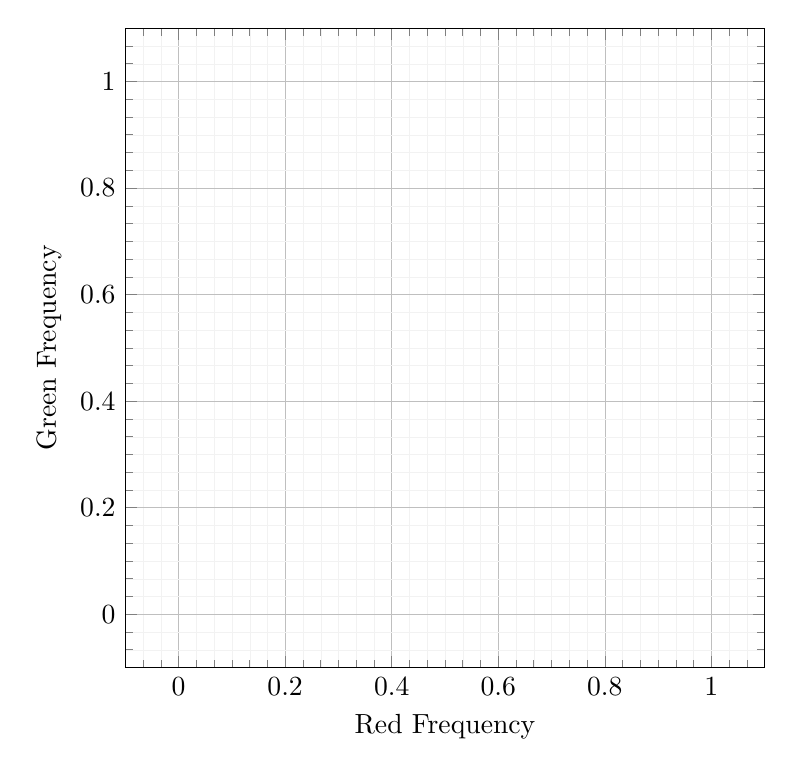
\begin{tikzpicture}
        \begin{axis}[
            xlabel={Red Frequency},
            ylabel={Green Frequency},
            zlabel={Blue Frequency},
            xlabel style={sloped like x axis}, % Make x label follow the x axis
            ylabel style={sloped like y axis}, % Make y label follow the y axis
            zlabel style={sloped}, % Make z label follow the z axis or make it vertical
            legend pos=north west,
            grid=both,
            grid style={line width=.1pt, draw=gray!10},
            major grid style={line width=.2pt,draw=gray!50},
            minor tick num=5,
            width=0.8\textwidth,
            height=0.8\textwidth,
            view={-80}{45}, % Adjust the view angle for better visualization
        ]
        \IfFileExists{code/output_data/color_sensor_calibration/rightColor.csv}{

            % SEEN point
            \addplot3[only marks, ball color=\seencolor, mark=ball, mark size = \ballsize*1.3, draw opacity = 0] coordinates {(\seenx, \seeny, \seenz)};
            \addlegendentry{Frequencies Read by Sensor}

            % CALIBRATION point
            \addlegendentry{Closest Calibration Point \& Used Color}
            \addplot3[only marks, ball color=blue, mark=ball, mark size = \ballsize*1.3, draw opacity = 1, draw= \seencolor, line width = 0.5mm] coordinates {(\calix, \caliy, \caliz)};

            % Line between the two
            \addplot3[ no marks,thick, line width=0.5mm, color=\seencolor, opacity = 1, -latex] coordinates {(\seenx, \seeny, \seenz) (\calix, \caliy, \caliz)};

            % Determine opacity based on sensor

            \addplot3[
                only marks,
                scatter,
                scatter/classes={
                    RED={mark=ball,ball color= red, draw opacity=0, mark size = 0},
                    BLUE={mark=ball,ball color= blue, draw opacity=0, mark size = \ballsize},
                    GREEN={mark=ball,ball color= green, draw opacity=0, mark size = 0},
                    WHITE={mark=ball,ball color= white, draw opacity=0, mark size = 0},
                    BLACK={mark=ball,ball color= black, draw opacity=0, mark size = \ballsize},
                    YELLOW={mark=ball,ball color= yellow, draw opacity=0, mark size = 0}
                },
                scatter src=explicit symbolic,
            ] table[
                x=Red_Freq,
                y=Green_Freq,
                z=Blue_Freq,
                meta = Color,
                col sep=comma,
            ] {code/output_data/color_sensor_calibration/rightColor.csv};

            % Wall histogram on the left
            \addplot3[
                only marks,
                scatter,
                scatter/classes={
                    RED={mark=*,fill=gray, fill opacity=0, draw opacity=0},
                    BLUE={mark=*,fill=gray, fill opacity=\grayopacity, draw opacity=0},
                    GREEN={mark=*,fill=gray, fill opacity=0, draw opacity=0},
                    WHITE={mark=*,fill=gray, fill opacity=0, draw opacity=0},
                    BLACK={mark=*,fill=gray, fill opacity=\grayopacity, draw opacity=0},
                    YELLOW={mark=*,fill=gray, fill opacity=0, draw opacity=0}
                },
                scatter src=explicit symbolic,
            ] table[
                x = Red_Freq,  % This sets the x-coordinate to 0
                y expr = 800,  % This sets the y-coordinate to 0
                z= Blue_Freq,
                meta = Color,
                col sep=comma,
            ] {code/output_data/color_sensor_calibration/rightColor.csv};

            % Wall histogram on the right
            \addplot3[
                only marks,
                scatter,
                scatter/classes={
                    RED={mark=*,fill=gray, fill opacity=0, draw opacity=0},
                    BLUE={mark=*,fill=gray, fill opacity=\grayopacity, draw opacity=0},
                    GREEN={mark=*,fill=gray, fill opacity=0, draw opacity=0},
                    WHITE={mark=*,fill=gray, fill opacity=0, draw opacity=0},
                    BLACK={mark=*,fill=gray, fill opacity=\grayopacity, draw opacity=0},
                    YELLOW={mark=*,fill=gray, fill opacity=0, draw opacity=0}
                },
                scatter src=explicit symbolic,
            ] table[
                x expr = 750,  % This sets the x-coordinate to 0
                y = Green_Freq,  % This sets the y-coordinate to the back wall
                z= Blue_Freq,
                meta = Color,
                col sep=comma,
            ] {code/output_data/color_sensor_calibration/rightColor.csv};

            % Floor histogram
            \addplot3[
                only marks,
                scatter,
                scatter/classes={
                    RED={mark=*,fill=gray, fill opacity=0, draw opacity=0},
                    BLUE={mark=*,fill=gray, fill opacity=\grayopacity, draw opacity=0},
                    GREEN={mark=*,fill=gray, fill opacity=0, draw opacity=0},
                    WHITE={mark=*,fill=gray, fill opacity=0, draw opacity=0},
                    BLACK={mark=*,fill=gray, fill opacity=\grayopacity, draw opacity=0},
                    YELLOW={mark=*,fill=gray, fill opacity=0, draw opacity=0}
                },
                scatter src=explicit symbolic,
            ] table[
                x = Red_Freq,
                y = Green_Freq,
                z expr = 0,
                meta = Color,
                col sep=comma,
            ] {code/output_data/color_sensor_calibration/rightColor.csv};

            
        }{}
        \end{axis}
    \end{tikzpicture}
    \caption{Visual representation of color matching algorithm. The orange dot is the seen color by the sensor, and the nearest calibration point is blue, thus the color seen is set to blue.}
    \label{fig:color-calibration-distance-example}
\end{figure}

\end{document}

            % SEEN point on bottom wall
            \addplot3[only marks, mark = *, fill = \seencolor,fill opacity = \shadowopacity, draw opacity = 0, mark size = \ballsize*0.9] coordinates {(\seenx, \seeny, 0)};

            % CALIBRATION point on bottom wall
            \addplot3[only marks, mark = *, fill = \calicolor,fill opacity = \shadowopacity, draw opacity = 0, mark size = \ballsize*0.9] coordinates {(\calix, \caliy, 0)};

            % Line on bottom wall
            \addplot3[ no marks,thick, line width=0.5mm, color=\seencolor, opacity = \shadowopacity, -latex] coordinates {(\seenx, \seeny, 0) (\calix, \caliy, 0)};

            % SEEN point on right wall
            \addplot3[only marks, mark = *, fill = \seencolor,fill opacity = \shadowopacity, draw opacity = 0, mark size = \ballsize*0.9] coordinates {(\maxx, \seeny, \seenz)};

            % CALIBRATION point on right wall
            \addplot3[only marks, mark = *, fill = \calicolor,fill opacity = \shadowopacity, draw opacity = 0, mark size = \ballsize*0.9] coordinates {(\maxx, \caliy, \caliz)};

            % Line on right wall
            \addplot3[ no marks,thick, line width=0.5mm, color=\seencolor, opacity = \shadowopacity, -latex] coordinates {(\maxx, \seeny, \seenz) (\maxx, \caliy, \caliz)};


\subsection{Ultrasonic Sensors}
The code is found in \cref{lst:ultrasonic-h}. The 3 ultrasonic sensors had 2 different uses. The outer ultrasonic sensors were used in the obstacle avoidance testing, allowing for the vehicle to sense when an obstacle was blocking the vehicle, and become parallel. The sensor mounts allowed for these ultrasonic sensors to be wider than the wheels allowing the vehicle to not hit the obstacles on passing, due to the nature of how the sensors project. If the ultrasonic sensors sensed something was in the way, the vehicle was programmed to move sideways until it found a way through. 

\par The central ultrasonic sensor was used to recognize the distance from the vehicle to the platform for the box pickup and placement. This allowed the vehicle to get to the best possible distance for the gripper to grab the box effectively and allow the button on the box to be pressed.

\subsection{IR Array sensor}
The \gls{IR} array sensor was used to determine the ``centeredness'' on a line. Since the \gls{IR} array was placed in the middle of the vehicle, (seen in \cref{fig:underside}), if the \gls{IR} array had it's middle sensors activated, the vehicle was correctly following the line. If the sensors on the right of the \gls{IR} array were activated, the vehicle would correct and move to the right. If the sensors on the left of the \gls{IR} array were activated, the vehicle would correct and move to the left. This was implemented as the best form of line following due to the inconsistencies of the color sensors as a line following mechanism. Additionally, each tape color had a slightly different value returned from each sensor, and thus calibration points were taken for each color individually, seen in \cref{ir-calibration-data}.

\par The algorithm to determine the ``centerdness'' of the sensor based on which sensors on the array were lit up was somewhat involved. The \gls{IR} sensors would return either a $1$ or a $0$ depending on if they sensed a line or not. This was then weighted based on their position on the array, with the sensors on the edges of the array receiving a higher weighting than the center. The left sensors were weighted negative and the right sensors were weighted positive. Additionally, it was designed that if just the leftmost sensor was activated, it would be $-1$, and if just the rightmost sensor was activated, the error would return $+1$. The left sensors had their value averaged and the right sensors had their value averaged, and then summed. Thus, the maximum magnitude of the reading would be $1$. The mathematical description of this was derived by Max Westerman and is shown below.

\[
w_i = \begin{cases} 
  (-1 + 2 \cdot \frac{i}{N-1}) & \text{if triggered}(i) = 1 \\
  0 & \text{otherwise}
\end{cases}
\]

\[
\text{leftPoint} = \left\lfloor \frac{N-1}{2} \right\rfloor, \quad \text{rightPoint} = \left\lceil \frac{N}{2} \right\rceil
\]

\[
\text{sumLeftWeight} = \sum_{i=0}^{\text{leftPoint}} w_i, \quad \text{countLeftWeight} = \sum_{i=0}^{\text{leftPoint}} 1 \text{ if } w_i \neq 0
\]

\[
\text{sumRightWeight} = \sum_{i=\text{rightPoint}}^{N-1} w_i, \quad \text{countRightWeight} = \sum_{i=\text{rightPoint}}^{N-1} 1 \text{ if } w_i \neq 0
\]

\[
\text{avgLeftWeight} = \frac{\text{sumLeftWeight}}{\text{countLeftWeight}} \text{ if } \text{countLeftWeight} > 0 \text{ else } 0
\]

\[
\text{avgRightWeight} = \frac{\text{sumRightWeight}}{\text{countRightWeight}} \text{ if } \text{countRightWeight} > 0 \text{ else } 0
\]

\[
\text{error} = \text{avgLeftWeight} + \text{avgRightWeight}
\]

\subsection{Gripper Button}
The mechanism of the gripper button allowed the robot to know what size box it was handling. When the gripper started to close around the box, a timer was started. When the button was activated by the box pressing against it, the timer stopped. If this time was below a certain threshold, the box was deemed to be a large box. If this time was above a certain threshold, the box was deemed to be a small box. 

\subsection{Pickup \& Place Flowchart}

The flow chart was split up into multiple sub modules seen in red so that it could be broken up into multiple pages. The red circle and hexagons designate these sub modules. Additionally, ``functions'' have been created with the green color, which take inputs from the sub modules as variables, seen in thicker arrows. See \cref{sc:pickup-place-flowchart} for the flowcharts.

\subsection{Structure}

The code was split up into multiple \texttt{.h} files and then imported into the main file. This was done to create a modular file system and easily isolate specific pieces of code from one another, just by not importing a file in the \texttt{main.ino}. The sensors were independent of one another and thus were placed in their own sub-directory, while the code that was built upon the sensors, such as line following, obstacle avoidance, robot movement, etc. was kept in the main folder.

\begin{figure}[H]
    \centering
    \begin{minipage}{0.4\textwidth}
        \dirtree{%
        .0 .
        .1 main.
        .2 main.ino.
        .2 BoxControl.h.
        .2 Initialization.h.
        .2 LineFollowing.h.
        .2 Motion.h.
        .2 ObstacleAvoidance.h.
        .2 PickupPlace.h.
        .2 controls.
        .3 PIDController.h.
        .3 Utils.h.
        .2 sensors.
        .3 Button.h.
        .3 ColorSensor.h.
        .3 IRSensorArray.h.
        .3 MWServo.h.
        .3 Motor.h.
        .3 UltraSonic.h.
        .1 readme.md.
        }
    \end{minipage}
    \caption{Code Directory Tree}
    \label{fig:code-directory-tree}
\end{figure}

\end{document}
\documentclass[11pt]{report}
\usepackage{StyleSheets/main}
\begin{document}

\chapter{System Test and Verification}\label{ch:system-test}

{
\footnotesize
\begin{longtable}{|R{2.8cm}|M{2.2cm}|M{2.4cm}|M{2.6cm}|M{0.7cm}|R{3cm}|}
\caption{Verification and Validation Requirements} \label{tab:long_table} \\
\hline \hline
\multirow{2}{3.5cm}{\textbf{Element / Component}} & 
\multirow{2}{*}{\textbf{Requirement}} & 
\multicolumn{3}{c|}{\textbf{Verification \& Validation Methods}} & 
\multirow{2}{3.5cm}{\textbf{Analysis}} \\ \cline{3-5} 
 & 
 & 
\textbf{Inspection} & 
\textbf{Demonstration} & 
\textbf{Test} & 
\\ \hline
\endfirsthead


\multicolumn{6}{c}%
{{\bfseries \tablename\ \thetable{} -- continued from previous page}} \\
\hline
\multirow{2}{3.5cm}{\textbf{Element / Component}} & 
\multirow{2}{*}{\textbf{Requirement}} & 
\multicolumn{3}{c|}{\textbf{Verification \& Validation Methods}} & 
\multirow{2}{3.5cm}{\textbf{Analysis}} \\ \cline{3-5} 
 & 
 & 
\textbf{Inspection} & 
\textbf{Demonstration} & 
\textbf{Test} & 
\\ \hline
\endhead

\hline \multicolumn{6}{|r|}{{Continued on next page}} \\ \hline
\endfoot

\hline \hline
\endlastfoot

% Insert your data here
Box Pickup-and-Placement System & \crefnum{sub:recognition-of-the-i-beam} & \checkmark & & \checkmark & \Cref{tst:location-of-box} -- Location of Box \\
\cline{2-6}
& \crefnum{sub:orientation-of-the-i-beam} & \checkmark & & & \Cref{tst:location-of-box} -- Location of Box \\
\cline{2-6}
& \crefnum{sub:apprehend-the-box} & \checkmark & & \checkmark & \Cref{tst:pickup-of-box} -- Pickup of Box \\
\cline{2-6}
& \crefnum{sub:identify-the-color-of-the-box} & \checkmark & & \checkmark & \Cref{tst:pickup-of-box} -- Pickup of Box \\
\cline{2-6}
& \crefnum{sub:identify-the-size-of-the-box} & \checkmark & & \checkmark & \Cref{tst:pickup-of-box} -- Pickup of Box \\
\cline{2-6}
& \crefnum{sub:realign-with-the-line-following-course} & \checkmark & & \checkmark & \Cref{tst:line-box-following} -- Line Box Following \\
\cline{2-6}
& \crefnum{sub:follow-the-line-of-the-color-of-the-box-and-return} & & & & \Cref{tst:line-box-following} -- Line Box Following \\
\cline{2-6}
& \crefnum{sub:placement-of-the-box} & \checkmark & & \checkmark & \Cref{tst:line-box-following} -- Line Box Following \\
\hline
\multirow{-3}{*}{Drive Train} & \crefnum{sub:move-forward} & \checkmark & & \checkmark & \Cref{tst:basic-directional-movement} -- Basic Directional Movement \\
\cline{2-6}
& \crefnum{sub:move-backward} & \checkmark & & \checkmark & \Cref{tst:basic-directional-movement} -- Basic Directional Movement \\
\cline{2-6}
& \crefnum{sub:move-right} & \checkmark & & \checkmark & \Cref{tst:basic-directional-movement} -- Basic Directional Movement \\
\cline{2-6}
& \crefnum{sub:move-left} & \checkmark & & \checkmark & \Cref{tst:basic-directional-movement} -- Basic Directional Movement \\
\cline{2-6}
\multirow{-2}{*}{Drive Train cont.} & \crefnum{sub:rotational-movement} & \checkmark & & \checkmark & \Cref{tst:rotational-movement} -- Rotational Movement \\
\hline
\multirow{-2}{*}{IR Sensor} & \crefnum{sub:width-of-the-ir-sensors} & \checkmark & & & \Cref{tst:ir-array-observation} -- \gls{IR} Array Observation \\
\cline{2-6}
& \crefnum{sub:the-number-of-sensors-is-greater-than-6} & \checkmark & & & \Cref{tst:ir-array-observation} -- \gls{IR} Array Observation \\
\cline{2-6}
& \crefnum{sub:it-must-detect-and-distinguish-the-tape-and-tarp} & \checkmark & & \checkmark & \Cref{tst:ir-array-detection} -- \gls{IR} Array Detection \\
\cline{2-6}
& \crefnum{sub:it-must-be-able-to-calculate-error} & \checkmark & & \checkmark & \Cref{tst:ir-array-detection} -- \gls{IR} Array Detection \\
\cline{2-6}
& \crefnum{sub:deviation-adjustment} & \checkmark & & \checkmark & \Cref{tst:ir-array-movement} -- \gls{IR} Array Movement \\
\hline
\multirow{-3}{*}{Obstacle Avoidance} & \crefnum{sub:detection-of-walls} & \checkmark & & \checkmark & \Cref{tst:avoidance-of-boundaries-of-walls} -- Avoidance of Boundaries of Walls \\
\cline{2-6}
& \crefnum{sub:avoidance-of-walls} & \checkmark & & \checkmark & \Cref{tst:avoidance-of-boundaries-of-walls} -- Avoidance of Boundaries of Walls \\
\cline{2-6}
& \crefnum{sub:detection-of-side-boundaries-of-obstacle-course-via-color-sensors} & \checkmark & & \checkmark & \Cref{tst:color-sensing-for-side-boundaries} -- Color Sensing For Side Boundaries \\
\cline{2-6}
 & \crefnum{sub:stay-within-the-obstacle-course-until-course-is-complete} & \checkmark & & \checkmark & \Cref{tst:color-sensing-for-side-boundaries} -- Color Sensing For Side Boundaries \\
\cline{2-6}
 & \crefnum{sub:detection-of-the-finish-line-of-obstacle-course-via-color-sensors} & \checkmark & & \checkmark & \Cref{tst:color-sensing-for-end-boundaries} -- Color Sensing For End Boundary \\
\cline{2-6}
 & \crefnum{sub:system-stops-at-the-end-of-the-course} & \checkmark & & \checkmark & \Cref{tst:color-sensing-for-end-boundaries} -- Color Sensing For End Boundary \\
\end{longtable}
\scriptsize
}

\test{Location of Box}\label{tst:location-of-box}
\Cref{sub:recognition-of-the-i-beam,sub:orientation-of-the-i-beam} of the project were put in place to make the vehicle identify where the location of the I-beam is and to align the center of the system with the I-beam so the vehicle shall successfully pick up and place the box. These requirements were verified via inspection by watching the vehicle perform and by testing. The test was a type 2 test. The expected result of this test is that the vehicle shall move forward until the I-beam is detected and the vehicle will center itself in the middle of the I-beam. The vehicle was placed on a black tarp, the front end facing the I-beam. The I-beam is 20 inches in front of the vehicle, slightly off to the vehicle’s left. The USB connected the battery to the Teensy 4.1 board. The \texttt{PickupPlace} code in Arduino was then verified and uploaded. The battery is then turned on and the test begins. 

It was observed that the vehicle deviated off center and once the system detected the I-beam, the vehicle was to the right of the I-beam. The vehicle then moved forward, but it was not centered with the I-beam. The left motor speed was then adjusted slightly and an \gls{IR} sensor array was added to the bottom of the front part of the vehicle. The test was ran again 3 more times and it was observed that the centering of vehicle improved dramatically. However the system’s ability to detect the I-beam was still not meeting standards. It was then decided that using the left and right ultrasonic sensors was not bringing the accuracy and precision that was needed. A middle ultrasonic is then added in front of the front omni-wheel. The test is then ran again and it was observed that rhe vehicle then moved forward and was able to stay on a straight line and once the middle front sensor reached its trigger point it would start. After making these adjustments, the test and \cref{sub:recognition-of-the-i-beam,sub:orientation-of-the-i-beam} were then deemed successful.

\test{Pickup of Box}\label{tst:pickup-of-box}
\Cref{sub:apprehend-the-box} of the project state that the vehicle shall apprehend the box with the gripper. \Cref{sub:identify-the-color-of-the-box,sub:identify-the-size-of-the-box} identifying the color and size of the box also were able to be included in this test. These requirements were verified via inspection by watching the vehicle perform and by testing. The test was a type 2 test. The expected result of this test is that once the vehicle has arrived to the platform, centered itself with the platform, and lowered the gripper arm, the gripper shall apprehend the box and the examiner will be able to tell via the serial monitor the color of the box and the size of the box. Another aspect of this test was making sure the pushbuttons would click when it makes contact with the box. The 2 pushbutton are attached to the inside of the gripper finger clicked. The purpose of the pushbutton were to make sure the gripper finger stopped closing once it had apprehended the box and not squeeze the box. The gripper arm would then rise and the test would be deemed complete.  The blue and red boxes are then held between the fingers of the gripper where a color sensor is placed, and the color sensor is calibrated for the test. The vehicle was placed on a black tarp that has a green line. The vehicle is placed on top of a green line parallel to the I-beam, the front end of the vehicle faced the I-beam. A red box is placed on top of the I-beam. The I-beam is 20 inches in front of the vehicle, slightly off to the vehicle’s left. The USB connected the battery to the Teensy 4.1 board. The \texttt{PickupPlace} code in Arduino was then verified and uploaded. The battery is then turned on and the test begins. 

It is observed that the system moves forward and is centered itself with the I-beam. The gripper arm then lowers, however it does not lower enough that the gripper fingers are in between the box, the gripper fingers then close and the arm raises. The first adjustment that is made is the gripper arm angle. This is a line of code that determine how low or high the gripper arm will go. The gripper arm angle is adjusted and then test is ran again. It is then observed that system moves forward and is centred itself with the I-beam. The gripper arm then lowers the proper amount and the box is between the gripper fingers. The gripper finger closes and picks up the box successfully. It was also observed that the pushbutton did click. Another observation is made via observing the serial monitor on Arduino is that the color sensors and timing algorithm are working properly thus the correct color of the box can be detected and the time it takes the gripper to close can be record. The test is then ran 2 more times to check for consistency and it is observed that both times the pushbutton did not click. An adjustment is then made to the gripper finger which is removing the front pushbutton. The test is then ran 2 more times and 
\cref{sub:apprehend-the-box,sub:identify-the-size-of-the-box,sub:identify-the-color-of-the-box} are all met as well as the consistency of the pushbutton.

\test{Line Box Following}\label{tst:line-box-following}
\Cref{sub:realign-with-the-line-following-course} of the project states that the vehicle shall realign itself with the line following course. This must be done after apprehending the box and identifying the size and color of the box, thus for this test, it is assumed that \cref{sub:recognition-of-the-i-beam,sub:orientation-of-the-i-beam,sub:apprehend-the-box,sub:identify-the-size-of-the-box,sub:identify-the-color-of-the-box} are deemed complete. This test shall also check \cref{sub:follow-the-line-of-the-color-of-the-box-and-return,sub:placement-of-the-box}. These requirements were verified via inspection by watching the vehicle perform the line box following testing. The test was a type 2 test. The expected result of this test is once the vehicle has arrived to the platform, centered itself with the platform, lowered the gripper arm, apprehended the box, and determined the color and size of the box, the system will move backward until it has sensed a green line. It will then center itself over the green line, rotate the front of the vehicle to the side of the line that correlates to the box color, which will be blue or red for this project, and follow the green line to start of the red or blue line. It will then rotate onto the blue or red line and follow it to the other end of the course where it will be place it on a specific I-beam based on the size of the box. The vehicle was placed on a black tarp that has a green line. The vehicle is placed on top of a green line parallel to the I-beam, the front end of the vehicle faced the I-beam. A ‘big’ red box is placed on top of the I-beam. The USB connected the battery to the Teensy 4.1 board. The \texttt{PickupPlace} code in Arduino was then verified and uploaded. The battery is then turned on and the test begins. 

It was observed that the vehicle did arrived to the platform, centered itself with the platform, lowered the gripper arm, apprehended the box, and determined the color and size of the box, the system then moved backward until it has sensed a green line. It then centered itself over the green line, rotated the front of the vehicle to the side of the red line and moved forward on the green line to the beginning of the red line. The rotation onto the red line and its ability to stay straight on the red line was lacking. The system would make it all the way to the fork of the red tape where the red line split into two lines and the vehicle was to follow one of them depending on the size of the box. Once it reached that point it was not able to stop and move horizontally in the proper manner which is key for \cref{sub:placement-of-the-box}. The vehicle was also have issues centering itself over the red line and it was determined as well that the systems ability to consistently put itself over the green line to the standard we expected was not being met. It was then decided that a color sensor needed to be added to the front of the vehicle on the bottom side. This was put in to help center the vehicle on the green, red, and blue lines of tape and identify the fork of the red or blue tape. Another adjustment that was added was to vehicle was vehicle was an \gls{IR} Array. After the color sensor was calibrated and the \gls{IR} array was tested, the line box following test was ran again. It was observed that the vehicle did arrived to the platform, centered itself with the platform, lowered the gripper arm, apprehended the box, and determined the color and size of the box, the system then moved backward until it has sensed a green line. It then centered itself over the green line, rotated the front of the vehicle to the side of the red line and moved forward on the green line to the beginning of the red line. The vehicle then geometrically centered over the red line, rotated onto the red line and did not get off track. It then followed the red line all the way to fork of red tape, stopped when it was supposed to, moved to the right, followed the red tape forward, sensed the I-beam, placed the box back on the I-beam. It then raised the gripper arm slightly, rotated 180 degrees and followed the red line back to the start of the red line. 

\test{Basic Directional Movement}\label{tst:basic-directional-movement}
This test is set up to complete \cref{sub:move-forward,sub:move-backward,sub:move-right,sub:move-left} which are the foundation of the project by being able to move in all directions. These requirements were verified via inspection by watching the vehicle perform and by testing. The test was a type 1 test. The expected result is that the vehicle’s left, right, front, and rear wheel shall rotate forward and backwards half a second each and then after all 4 wheels rotate the vehicle shall move forward for 3 seconds, and stop. Then move backwards for 3 seconds, and stop. It would next move right for 3 seconds, and stop. Then move left for 3 seconds, and stop. The vehicle was placed on the floor. The USB connected the battery to the Teensy 4.1 board. A method in the code, \texttt{motorTest()}, under the class \texttt{Motor}, was then verified and uploaded. The battery is then turned on and the test begins. The code is found in \cref{lst:motor-h}.

It was observed that the vehicle’s left, right, front, and rear wheel rotated forward and backwards half a second each move forward for 3 seconds, and stop. Then the vehicle moved forward for 3 seconds and stopped. It then moved backwards for 3 seconds, and stop. It next moved right for 3 seconds, and stop. Then moved left for 3 seconds, and stop. The test and requirements \cref{sub:move-forward,sub:move-backward,sub:move-right,sub:move-left} were then deemed successful.

\test{Rotational Movement}\label{tst:rotational-movement}
This test is set up to complete \cref{sub:rotational-movement}. This requirements was verified via inspection by watching the vehicle perform and by testing. The test was a type 1 test. The expected result is that the vehicle shall follow a piece of red tape that is straight for the first 2 and a half feet and then veers 45 degrees to the right. The vehicle was placed on a black tarp at the beginning of the red tape, with the front of the vehicle facing the red tape. The USB connected the battery to the Teensy 4.1 board. The code within \gls{IR} class Arduino was then verified and uploaded, seen in \cref{lst:irsensorarray-h}. The battery is then turned on and the test begins. 

It was then observed that the vehicle would move straight forward on the red tape but when it encountered the red tape at the 45 degree angle, the vehicle was over rotating and unable to rotate onto the centerline. One adjustment that was made was to change the speed of the front and back motors. Another change that was made was to the \gls{IR} array sensor and how the vehicle used the error data the array produced. After the test was run 3 more times and the motor speeds were changed, it was observed that the vehicle would move straight forward on the red tape and  then encountered the red tape, it would properly rotate to the center of the red tape at a 45 degree line. Test and \cref{sub:rotational-movement} were deemed complete. 

\test{IR Array Observation}\label{tst:ir-array-observation}
\Cref{sub:width-of-the-ir-sensors,sub:the-number-of-sensors-is-greater-than-6} were completed via inspection. The \gls{IR} Array was scaled against the tape that is used for the courses. It was deemed it was the bigger than the size of the tape in terms of width. The number of sensors was also deemed to be greater than 6. \Cref{sub:width-of-the-ir-sensors,sub:the-number-of-sensors-is-greater-than-6} were completed. 

\test{IR Array Detection}\label{tst:ir-array-detection}
\Cref{sub:it-must-detect-and-distinguish-the-tape-and-tarp} is completed via inspection and testing. The \gls{IR} Array is attached to the button of the vehicle and connected to the Teensy 4.1 board via wires. The expected result of this test is that the vehicle will move as straight as possible on a red line of tape. The serial monitor will be observed at the same time of the vehicle’s movement. It is expected that once the vehicle begins to deviate right or left the values the serial monitor will change from what they were when the vehicle was moving straight. The vehicle is placed at the beginning of a straight piece of red tape, 30 inches long. The USB connected the battery to the Teensy 4.1 board. The \gls{IR} Array Test code is uploaded and verified. The battery is then turned on and the test begins. 

It is observed that the values of the serial monitor are changing when a sensor is over the tape compared to the black tarp. When the left arrays deviate to the left off the red tape their values become less than zero and when the right sensors deviate to the right off the tape, their values are greatest than zero. It is deemed \cref{sub:it-must-detect-and-distinguish-the-tape-and-tarp} is complete. 



Test 7 is also completed in this this test by adding code that sums of the average values of the right sensors and add that value to the sum of the left array values. We are able to tell with that value if the vehicle is deviating left of right. If the value is negative it’s beginning to yaw to the left and if the value is positive we know it is beginning to yaw to the right. 

The updated code is verified and uploaded, the test is ran again. The vehicle moved forward on the red line and began to deviate to the left and a negative error was observed on the serial monitor. It was deemed test 7.

\test{IR Array Movement}\label{tst:ir-array-movement}
The \gls{IR} array movement test is set to complete \cref{sub:it-must-be-able-to-calculate-error}. The expected result of this test is that the vehicle shall correct its deviation by turning back onto the line. The test will be on a green, blue, and red line. The rate of how much the vehicle turns is based on the absolute value of the error. The further away the error is from zero the more it will turn. The vehicle is placed at the beginning of a straight piece of red tape, 30 inches long. The USB connected the battery to the Teensy 4.1 board. The \gls{IR} Array deviation Test code is uploaded and verified. The battery is then turned on and the test begins. 

It is observed that the vehicle moved forward and deviated to the right and gave an error value of 0.4 when it began to drift to the right. It was then observed however that the amount the system corrected itself to the left was not enough thus it did not put itself back on the red tape. It was then decided that the proportional gain needed to be adjusted by increasing the value. The code was then updated and the test was then ran again. This test run the system drifted to the left and the error value as it first began to deviate from the line was $-0.2$, it then corrected it path by the correct amount of rotation. This was then tested on a green and blue line as well and no issues were found. \Cref{sub:it-must-be-able-to-calculate-error} was deemed complete.


\test{Avoidance of Boundaries of Walls}\label{tst:avoidance-of-boundaries-of-walls}
\Cref{sub:detection-of-walls,sub:avoidance-of-walls} of the project were put in place to make the vehicle avoid all walls within the obstacle course. These requirements were verified via inspection by watching the vehicle perform and by testing. The test was a type 2 test. The expected result of this test is that the vehicle will move forward until a wall is detected at a trigger distance, then move left until the right sensor senses a gap. It will then move forward until a wall is detected at trigger distance and then move left again. It is also expected that the vehicle stays in a straight line when moving horizontally. The test would then be deemed complete. The vehicle was placed on a black tarp, the front end facing the obstacle course. Two walls were placed on the obstacle course, one on the left side and one on the right side, about 30 inches apart vertically.  The USB connected the battery to the Teensy 4.1 board. The obstacle code in Arduino was then verified and uploaded. The battery is then turned on and the test begins. 

It was observed that the vehicle would move forward property, move left properly, stay in a straight line when moving horizontally, and not hit the wall or obstacle when moving forward, however when a gap was sensed it would wait too long to move forward. This was then fixed by reducing the motor speed and decreasing the delay. After making these adjustments, the test and \cref{sub:detection-of-walls,sub:avoidance-of-walls} were then deemed successful.

\test{Color Sensing For Side Boundaries}\label{tst:color-sensing-for-side-boundaries}
\Cref{sub:detection-of-side-boundaries-of-obstacle-course-via-color-sensors} was tested in the color sensing test for the side boundaries. This requirement was verified via inspection by watching the vehicle perform and by testing. The test was a type 2 test. The expected result of this test is that it would move forward from the starting position, detect a wall, and then move left until it detected a white line and move in the opposite direction which would satisfy \cref{sub:stay-within-the-obstacle-course-until-course-is-complete}. The vehicle was placed on a black tarp, the front end facing the obstacle course. Two walls are placed side by side about 20 inches from the starting position. The USB connected the battery to the Teensy 4.1 board. This test assumes test 8 and \cref{sub:detection-of-walls,sub:avoidance-of-walls} are completed. The obstacle test code which includes the color sensing code and obstacle avoidance code in Arduino was then verified and uploaded. The battery is then turned on and the test begins.

It was then observed that the vehicle moved forward, detected a wall, and moved left until a white line was detected, however, the vehicle then oscillated over the white line and did not have the ability to move back to the right. It was then discovered that the color sensors did not clear the data from the previous loop of code and since this code was using average color values the sensor had seen, it was then realized the data needed to be cleared so it wouldn’t affect the next task. This adjustment was made to the code. The test was then run again in the same form. It was then observed that the vehicle moved forward, detected a wall, and moved left until a white line was detected then moved back to the right side of the obstacle course, detected a white line, and moved back to the left. After making these adjustments, the test and \cref{sub:detection-of-side-boundaries-of-obstacle-course-via-color-sensors} were then deemed successful.

\test{Color Sensing for End Boundaries}\label{tst:color-sensing-for-end-boundaries}
\Cref{sub:detection-of-the-finish-line-of-obstacle-course-via-color-sensors,sub:system-stops-at-the-end-of-the-course} was tested in the color sensing test for the end boundary. This requirement was verified via inspection by watching the vehicle perform and by testing. The test was a type 2 test. The expected result of this test is that it would move forward from the starting position, detect a green line, and then fully cross the green line where it would come to a complete stop which would satisfy \cref{sub:system-stops-at-the-end-of-the-course}. The vehicle was placed on a black tarp, about 15 inches from the end of green tape/end of the course. The USB connected the battery to the Teensy 4.1 board. The obstacle test code which includes the color sensing code in Arduino was then verified and uploaded. The battery is then turned on and the test begins.

It was then observed that the vehicle moved forward, and detected a green line, however, the vehicle then only moved about halfway across it. A delay function and a variable named VerticleBoxLength were added to the code to make the vehicle fully cross the line in a more accurate manner. The test was then run again and the vehicle detected a green line and fully crossed the line and then came to a complete stop. \Cref{sub:system-stops-at-the-end-of-the-course,sub:detection-of-the-finish-line-of-obstacle-course-via-color-sensors} were fulfilled, thus a successful test. 

\end{document}
\documentclass{report}
\usepackage{StyleSheet}
\begin{document}

\chapter{System Analysis \& System Performance Metrics}\label{ch:system-analysis}

\end{document}
\documentclass[11pt]{report}
\usepackage{StyleSheets/main}
\begin{document}

\chapter{Summary}\label{ch:summary}

\end{document}

\singlespacing
\microtypesetup{protrusion=false} % Kerning disabled
\printglossary[type=\acronymtype]
\microtypesetup{protrusion=true}  % Kerning Enabled

\appendix

\section*{Documentation Statement}
\begin{description}
    \item[Speed Motor \#1:] To make the robot faster, the gearboxes of dead speed motors were swapped out with our slower, torque motors. The team utilized \emph{Savannah Prouty's} dead speed motor.
    \item[Speed Motor \#2:] As above, the team utilized \emph{Duncan Wood's} dead speed motor for it's gearbox.
    \item[\gls{PID} Guidance:] Although it did not make it into the final robot, \emph{Carter Sorenson} introduced the group to the possibility of using \gls{PID} control for the robot.
    \item[Motor Mounts:] The team did not check our box correctly, resulting in missing motor mounts. \emph{Savannah Prouty} provided the team with her extra motor mounts.
\end{description}

\documentclass[12pt]{report}
\usepackage{StyleSheets/main}
\begin{document}

\chapter{Calibration Data}

\section{Color Sensor Calibration Points}
\label{sc:color-sensor-points}
\documentclass[12pt]{report}
\usepackage{GraphDefinitions}

\begin{document}

\foreach \sensor in {middleColor, rightColor, leftColor, gripperColor} {
    \ifthenelse{\equal{\sensor}{middleColor}}{ % Middle color shadow opacity
        \def\opacity{0.010}
    }{
        \def\opacity{0.055} % Non middle color shadow opacity
    }
    \def\ballsize{3pt} % Change the size of the balls
                
    \begin{figure}[H]
        \centering
        \begin{tikzpicture}
            \begin{axis}[
                xlabel={Red Frequency},
                ylabel={Green Frequency},
                zlabel={Blue Frequency},
                xlabel style={sloped like x axis}, % Make x label follow the x axis
                ylabel style={sloped like y axis}, % Make y label follow the y axis
                zlabel style={sloped}, % Make z label follow the z axis or make it vertical
                legend pos=north west,
                grid=both,
                grid style={line width=.1pt, draw=gray!10},
                major grid style={line width=.2pt,draw=gray!50},
                minor tick num=5,
                width=0.8\textwidth,
                height=0.65\textwidth,
                view={45}{45}, % Adjust the view angle for better visualization
            ]
            \IfFileExists{code/output_data/color_sensor_calibration/\sensor.csv}{
                % Determine opacity based on sensor

                \addplot3[
                    only marks,
                    scatter,
                    scatter/classes={
                        RED={mark=ball,ball color= red, draw opacity=0, mark size = \ballsize},
                        BLUE={mark=ball,ball color= blue, draw opacity=0, mark size = \ballsize},
                        GREEN={mark=ball,ball color= green, draw opacity=0, mark size = \ballsize},
                        WHITE={mark=ball,ball color= white, draw opacity=0, mark size = \ballsize},
                        BLACK={mark=ball,ball color= black, draw opacity=0, mark size = \ballsize},
                        YELLOW={mark=ball,ball color= yellow, draw opacity=0, mark size = \ballsize}
                    },
                    scatter src=explicit symbolic,
                ] table[
                    x=Red_Freq,
                    y=Green_Freq,
                    z=Blue_Freq,
                    meta = Color,
                    col sep=comma,
                ] {code/output_data/color_sensor_calibration/\sensor.csv};

                % Wall histogram on the left
                \addplot3[
                    only marks,
                    scatter,
                    scatter/classes={
                        RED={mark=*,fill=red, fill opacity=\opacity, draw opacity=0},
                        BLUE={mark=*,fill=blue, fill opacity=\opacity, draw opacity=0},
                        GREEN={mark=*,fill=green, fill opacity=\opacity, draw opacity=0},
                        WHITE={mark=*,fill=gray, fill opacity=\opacity, draw opacity=0},
                        BLACK={mark=*,fill=black, fill opacity=\opacity, draw opacity=0},
                        YELLOW={mark=*,fill=yellow, fill opacity=\opacity, draw opacity=0}
                    },
                    scatter src=explicit symbolic,
                ] table[
                    x expr = 0,  % This sets the x-coordinate to 0
                    y = Green_Freq,  % This sets the y-coordinate to 0
                    z= Blue_Freq,
                    meta = Color,
                    col sep=comma,
                ] {code/output_data/color_sensor_calibration/\sensor.csv};

                % Wall histogram on the right
                \addplot3[
                    only marks,
                    scatter,
                    scatter/classes={
                        RED={mark=*,fill=red, fill opacity=\opacity, draw opacity=0},
                        BLUE={mark=*,fill=blue, fill opacity=\opacity, draw opacity=0},
                        GREEN={mark=*,fill=green, fill opacity=\opacity, draw opacity=0},
                        WHITE={mark=*,fill=gray, fill opacity=\opacity, draw opacity=0},
                        BLACK={mark=*,fill=black, fill opacity=\opacity, draw opacity=0},
                        YELLOW={mark=*,fill=yellow, fill opacity=\opacity, draw opacity=0}
                    },
                    scatter src=explicit symbolic,
                ] table[
                    x = Red_Freq,  % This sets the x-coordinate to 0
                    y expr = 750,  % This sets the y-coordinate to the back wall
                    z= Blue_Freq,
                    meta = Color,
                    col sep=comma,
                ] {code/output_data/color_sensor_calibration/\sensor.csv};

                % Floor histogram
                \addplot3[
                    only marks,
                    scatter,
                    scatter/classes={
                        RED={mark=*,fill=red, fill opacity=\opacity, draw opacity=0},
                        BLUE={mark=*,fill=blue, fill opacity=\opacity, draw opacity=0},
                        GREEN={mark=*,fill=green, fill opacity=\opacity, draw opacity=0},
                        WHITE={mark=*,fill=gray, fill opacity=\opacity, draw opacity=0},
                        BLACK={mark=*,fill=black, fill opacity=\opacity, draw opacity=0},
                        YELLOW={mark=*,fill=yellow, fill opacity=\opacity, draw opacity=0}
                    },
                    scatter src=explicit symbolic,
                ] table[
                    x = Red_Freq,
                    y = Green_Freq,
                    z expr = 0,
                    meta = Color,
                    col sep=comma,
                ] {code/output_data/color_sensor_calibration/\sensor.csv};

                
            }{}
            \end{axis}
        \end{tikzpicture}
        \caption{\sensor \ Sensor Calibration Data in Euclidean Space.}
        \label{fig:\sensor_calibration_data}
    \end{figure}
}

\end{document}

\subsection{Color Sensor Euclidean Distance Visualization}
\label{sc:color-sensor-visualization}
\documentclass{article}
\usepackage{GraphDefinitions}

\begin{document}

\def\grayopacity{0.055}
\def\ballsize{3pt} % Change the size of the balls
\def\seencolor{orange}
\def\seenx{543}
\def\seeny{340}
\def\seenz{500}
\def\calix{574}
\def\caliy{271}
\def\caliz{435}
\def\calicolor{blue}
\def\maxy{750}
\def\maxx{825}
\def\shadowopacity{0.4}
            
\begin{figure}[H]
    \centering
    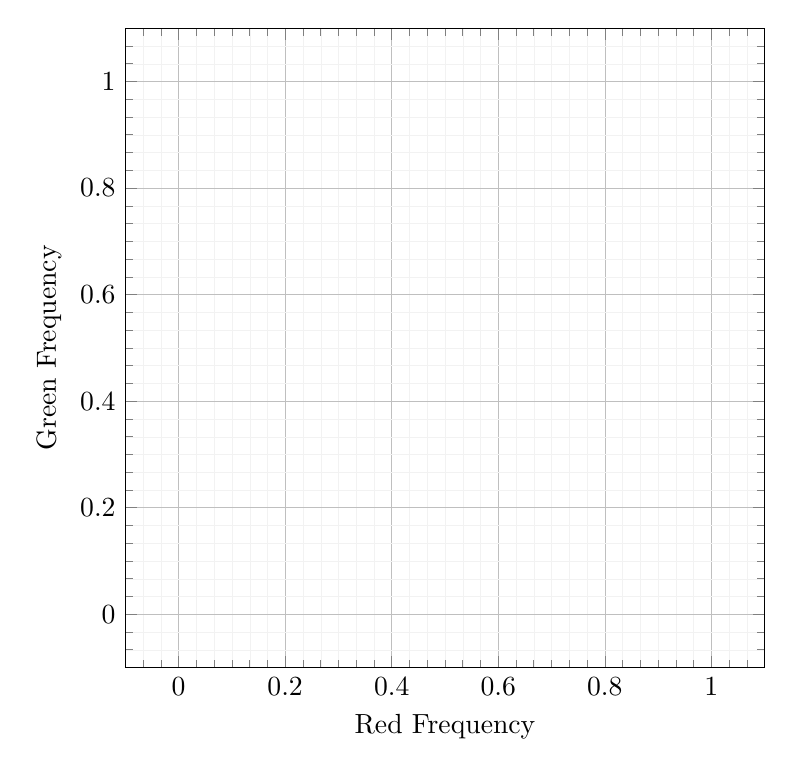
\begin{tikzpicture}
        \begin{axis}[
            xlabel={Red Frequency},
            ylabel={Green Frequency},
            zlabel={Blue Frequency},
            xlabel style={sloped like x axis}, % Make x label follow the x axis
            ylabel style={sloped like y axis}, % Make y label follow the y axis
            zlabel style={sloped}, % Make z label follow the z axis or make it vertical
            legend pos=north west,
            grid=both,
            grid style={line width=.1pt, draw=gray!10},
            major grid style={line width=.2pt,draw=gray!50},
            minor tick num=5,
            width=0.8\textwidth,
            height=0.8\textwidth,
            view={-80}{45}, % Adjust the view angle for better visualization
        ]
        \IfFileExists{code/output_data/color_sensor_calibration/rightColor.csv}{

            % SEEN point
            \addplot3[only marks, ball color=\seencolor, mark=ball, mark size = \ballsize*1.3, draw opacity = 0] coordinates {(\seenx, \seeny, \seenz)};
            \addlegendentry{Frequencies Read by Sensor}

            % CALIBRATION point
            \addlegendentry{Closest Calibration Point \& Used Color}
            \addplot3[only marks, ball color=blue, mark=ball, mark size = \ballsize*1.3, draw opacity = 1, draw= \seencolor, line width = 0.5mm] coordinates {(\calix, \caliy, \caliz)};

            % Line between the two
            \addplot3[ no marks,thick, line width=0.5mm, color=\seencolor, opacity = 1, -latex] coordinates {(\seenx, \seeny, \seenz) (\calix, \caliy, \caliz)};

            % Determine opacity based on sensor

            \addplot3[
                only marks,
                scatter,
                scatter/classes={
                    RED={mark=ball,ball color= red, draw opacity=0, mark size = 0},
                    BLUE={mark=ball,ball color= blue, draw opacity=0, mark size = \ballsize},
                    GREEN={mark=ball,ball color= green, draw opacity=0, mark size = 0},
                    WHITE={mark=ball,ball color= white, draw opacity=0, mark size = 0},
                    BLACK={mark=ball,ball color= black, draw opacity=0, mark size = \ballsize},
                    YELLOW={mark=ball,ball color= yellow, draw opacity=0, mark size = 0}
                },
                scatter src=explicit symbolic,
            ] table[
                x=Red_Freq,
                y=Green_Freq,
                z=Blue_Freq,
                meta = Color,
                col sep=comma,
            ] {code/output_data/color_sensor_calibration/rightColor.csv};

            % Wall histogram on the left
            \addplot3[
                only marks,
                scatter,
                scatter/classes={
                    RED={mark=*,fill=gray, fill opacity=0, draw opacity=0},
                    BLUE={mark=*,fill=gray, fill opacity=\grayopacity, draw opacity=0},
                    GREEN={mark=*,fill=gray, fill opacity=0, draw opacity=0},
                    WHITE={mark=*,fill=gray, fill opacity=0, draw opacity=0},
                    BLACK={mark=*,fill=gray, fill opacity=\grayopacity, draw opacity=0},
                    YELLOW={mark=*,fill=gray, fill opacity=0, draw opacity=0}
                },
                scatter src=explicit symbolic,
            ] table[
                x = Red_Freq,  % This sets the x-coordinate to 0
                y expr = 800,  % This sets the y-coordinate to 0
                z= Blue_Freq,
                meta = Color,
                col sep=comma,
            ] {code/output_data/color_sensor_calibration/rightColor.csv};

            % Wall histogram on the right
            \addplot3[
                only marks,
                scatter,
                scatter/classes={
                    RED={mark=*,fill=gray, fill opacity=0, draw opacity=0},
                    BLUE={mark=*,fill=gray, fill opacity=\grayopacity, draw opacity=0},
                    GREEN={mark=*,fill=gray, fill opacity=0, draw opacity=0},
                    WHITE={mark=*,fill=gray, fill opacity=0, draw opacity=0},
                    BLACK={mark=*,fill=gray, fill opacity=\grayopacity, draw opacity=0},
                    YELLOW={mark=*,fill=gray, fill opacity=0, draw opacity=0}
                },
                scatter src=explicit symbolic,
            ] table[
                x expr = 750,  % This sets the x-coordinate to 0
                y = Green_Freq,  % This sets the y-coordinate to the back wall
                z= Blue_Freq,
                meta = Color,
                col sep=comma,
            ] {code/output_data/color_sensor_calibration/rightColor.csv};

            % Floor histogram
            \addplot3[
                only marks,
                scatter,
                scatter/classes={
                    RED={mark=*,fill=gray, fill opacity=0, draw opacity=0},
                    BLUE={mark=*,fill=gray, fill opacity=\grayopacity, draw opacity=0},
                    GREEN={mark=*,fill=gray, fill opacity=0, draw opacity=0},
                    WHITE={mark=*,fill=gray, fill opacity=0, draw opacity=0},
                    BLACK={mark=*,fill=gray, fill opacity=\grayopacity, draw opacity=0},
                    YELLOW={mark=*,fill=gray, fill opacity=0, draw opacity=0}
                },
                scatter src=explicit symbolic,
            ] table[
                x = Red_Freq,
                y = Green_Freq,
                z expr = 0,
                meta = Color,
                col sep=comma,
            ] {code/output_data/color_sensor_calibration/rightColor.csv};

            
        }{}
        \end{axis}
    \end{tikzpicture}
    \caption{Visual representation of color matching algorithm. The orange dot is the seen color by the sensor, and the nearest calibration point is blue, thus the color seen is set to blue.}
    \label{fig:color-calibration-distance-example}
\end{figure}

\end{document}

            % SEEN point on bottom wall
            \addplot3[only marks, mark = *, fill = \seencolor,fill opacity = \shadowopacity, draw opacity = 0, mark size = \ballsize*0.9] coordinates {(\seenx, \seeny, 0)};

            % CALIBRATION point on bottom wall
            \addplot3[only marks, mark = *, fill = \calicolor,fill opacity = \shadowopacity, draw opacity = 0, mark size = \ballsize*0.9] coordinates {(\calix, \caliy, 0)};

            % Line on bottom wall
            \addplot3[ no marks,thick, line width=0.5mm, color=\seencolor, opacity = \shadowopacity, -latex] coordinates {(\seenx, \seeny, 0) (\calix, \caliy, 0)};

            % SEEN point on right wall
            \addplot3[only marks, mark = *, fill = \seencolor,fill opacity = \shadowopacity, draw opacity = 0, mark size = \ballsize*0.9] coordinates {(\maxx, \seeny, \seenz)};

            % CALIBRATION point on right wall
            \addplot3[only marks, mark = *, fill = \calicolor,fill opacity = \shadowopacity, draw opacity = 0, mark size = \ballsize*0.9] coordinates {(\maxx, \caliy, \caliz)};

            % Line on right wall
            \addplot3[ no marks,thick, line width=0.5mm, color=\seencolor, opacity = \shadowopacity, -latex] coordinates {(\maxx, \seeny, \seenz) (\maxx, \caliy, \caliz)};


\section{IR Array Calibration Points}
\label{sc:ir-array-points}
\documentclass{article}
\usepackage{GraphDefinitions}

\begin{document}

\begin{figure}[H]
\centering
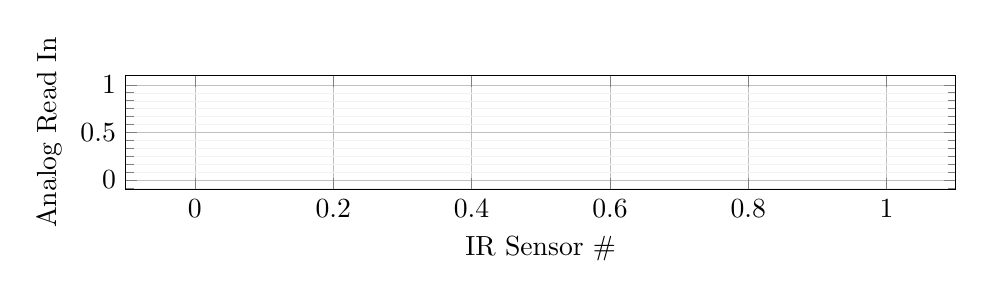
\begin{tikzpicture}
\begin{axis}[
    width=1\textwidth, % Adjust the width as needed
    height=0.25\textwidth, % Adjust the height as needed
    xlabel={IR Sensor \#},
    ylabel={Analog Read In},
    xtick={1, 2, 3, 4, 5, 6, 7}, % Set specific x-axis labels
    legend pos=north west,
    grid=both,
    grid style={line width=.1pt, draw=gray!10},
    major grid style={line width=.2pt,draw=gray!50},
    minor y tick num=5, % This adds the minor grid lines on the y-axis
    minor x tick num=0, % This removes the minor grid lines on the x-axis
    ]
    \IRTrace{green}{Green}{green}
    \IRTrace{blue}{Blue}{blue}
    \IRTrace{red}{Red}{red}
    \IRTrace{yellow}{Yellow}{black}
    \IRTrace{black}{Off}{black}
\end{axis}
\end{tikzpicture}
\caption{IR Calibration Data Based on Tape Color.}
\label{ir-calibration-data}
\end{figure}

\end{document}


\section{Motor Calibration Points}
\label{sc:motor-points}
\documentclass[12pt]{report}
\usepackage{GraphDefinitions}

\begin{document}

\begin{figure}[H]
\centering
\begin{tikzpicture}
    \begin{axis}[
        title = {Speed Percent ($\% \cdot 100$) vs Speed (cm/s)}
        width=\textwidth, % Make the plot as wide as the subfigure
        height=0.5\textwidth, % Adjust the height for a wide format
        xlabel={Speed (cm/s)},
        ylabel={Speed Percent ($\% \cdot 100$)},
        legend pos=north west,
        ymin = -10,
        grid=both,
        grid style={line width=.1pt, draw=gray!10},
        major grid style={line width=.2pt,draw=gray!50},
        ]
        \MotorTrace{left}{speed_percent}{Left Speed Percent}{red}{solid}        
        \MotorTrace{right}{speed_percent}{Right Speed Percent}{green}{solid}
        \MotorTrace{top}{speed_percent}{Top Speed Percent}{blue}{solid}
        \MotorTrace{bottom}{speed_percent}{Bottom Speed Percent}{black}{solid}
    \end{axis}
\end{tikzpicture}
\label{speed-calibration-data}
\caption{Motor Calibration Data Regarding Speed Percent}
\end{figure}

\vspace{0.5cm} % Space between the subfigures

\begin{figure}[H]
\centering
\begin{tikzpicture}
    \begin{axis}[
        title = {PWM Percent ($\% \cdot 100$) vs Speed (cm/s)}
        width=\textwidth, % Make the plot as wide as the subfigure
        height=0.5\textwidth, % Adjust the height for a wide format
        xlabel={Speed (cm/s)},
        ylabel={PWM Percent ($\% \cdot 100$)},
        ymin = -10,
        legend pos=north west,
        grid=both,
        grid style={line width=.1pt, draw=gray!10},
        major grid style={line width=.2pt,draw=gray!50},
        ]
        \MotorTrace{left}{pwm_percent}{Left PWM Percent}{red}{solid}        
        \MotorTrace{right}{pwm_percent}{Right PWM Percent}{green}{solid}
        \MotorTrace{top}{pwm_percent}{Top PWM Percent}{blue}{solid}
        \MotorTrace{bottom}{pwm_percent}{Bottom PWM Percent}{black}{solid}
    \end{axis}
\end{tikzpicture}
\label{pwm-calibration-data}
\caption{Motor Calibration Data Regarding PWM Percent}
\end{figure}

\end{document}


\end{document}
\documentclass[12pt]{report}
\usepackage{StyleSheets/main}
\begin{document}

\chapter{Diagrams}

\section{Robot Designs}

\subsection{Design 1}
\label{sc:color-sensor-points}
\documentclass[12pt]{report}
\usepackage{GraphDefinitions}

\begin{document}

\foreach \sensor in {middleColor, rightColor, leftColor, gripperColor} {
    \ifthenelse{\equal{\sensor}{middleColor}}{ % Middle color shadow opacity
        \def\opacity{0.010}
    }{
        \def\opacity{0.055} % Non middle color shadow opacity
    }
    \def\ballsize{3pt} % Change the size of the balls
                
    \begin{figure}[H]
        \centering
        \begin{tikzpicture}
            \begin{axis}[
                xlabel={Red Frequency},
                ylabel={Green Frequency},
                zlabel={Blue Frequency},
                xlabel style={sloped like x axis}, % Make x label follow the x axis
                ylabel style={sloped like y axis}, % Make y label follow the y axis
                zlabel style={sloped}, % Make z label follow the z axis or make it vertical
                legend pos=north west,
                grid=both,
                grid style={line width=.1pt, draw=gray!10},
                major grid style={line width=.2pt,draw=gray!50},
                minor tick num=5,
                width=0.8\textwidth,
                height=0.65\textwidth,
                view={45}{45}, % Adjust the view angle for better visualization
            ]
            \IfFileExists{code/output_data/color_sensor_calibration/\sensor.csv}{
                % Determine opacity based on sensor

                \addplot3[
                    only marks,
                    scatter,
                    scatter/classes={
                        RED={mark=ball,ball color= red, draw opacity=0, mark size = \ballsize},
                        BLUE={mark=ball,ball color= blue, draw opacity=0, mark size = \ballsize},
                        GREEN={mark=ball,ball color= green, draw opacity=0, mark size = \ballsize},
                        WHITE={mark=ball,ball color= white, draw opacity=0, mark size = \ballsize},
                        BLACK={mark=ball,ball color= black, draw opacity=0, mark size = \ballsize},
                        YELLOW={mark=ball,ball color= yellow, draw opacity=0, mark size = \ballsize}
                    },
                    scatter src=explicit symbolic,
                ] table[
                    x=Red_Freq,
                    y=Green_Freq,
                    z=Blue_Freq,
                    meta = Color,
                    col sep=comma,
                ] {code/output_data/color_sensor_calibration/\sensor.csv};

                % Wall histogram on the left
                \addplot3[
                    only marks,
                    scatter,
                    scatter/classes={
                        RED={mark=*,fill=red, fill opacity=\opacity, draw opacity=0},
                        BLUE={mark=*,fill=blue, fill opacity=\opacity, draw opacity=0},
                        GREEN={mark=*,fill=green, fill opacity=\opacity, draw opacity=0},
                        WHITE={mark=*,fill=gray, fill opacity=\opacity, draw opacity=0},
                        BLACK={mark=*,fill=black, fill opacity=\opacity, draw opacity=0},
                        YELLOW={mark=*,fill=yellow, fill opacity=\opacity, draw opacity=0}
                    },
                    scatter src=explicit symbolic,
                ] table[
                    x expr = 0,  % This sets the x-coordinate to 0
                    y = Green_Freq,  % This sets the y-coordinate to 0
                    z= Blue_Freq,
                    meta = Color,
                    col sep=comma,
                ] {code/output_data/color_sensor_calibration/\sensor.csv};

                % Wall histogram on the right
                \addplot3[
                    only marks,
                    scatter,
                    scatter/classes={
                        RED={mark=*,fill=red, fill opacity=\opacity, draw opacity=0},
                        BLUE={mark=*,fill=blue, fill opacity=\opacity, draw opacity=0},
                        GREEN={mark=*,fill=green, fill opacity=\opacity, draw opacity=0},
                        WHITE={mark=*,fill=gray, fill opacity=\opacity, draw opacity=0},
                        BLACK={mark=*,fill=black, fill opacity=\opacity, draw opacity=0},
                        YELLOW={mark=*,fill=yellow, fill opacity=\opacity, draw opacity=0}
                    },
                    scatter src=explicit symbolic,
                ] table[
                    x = Red_Freq,  % This sets the x-coordinate to 0
                    y expr = 750,  % This sets the y-coordinate to the back wall
                    z= Blue_Freq,
                    meta = Color,
                    col sep=comma,
                ] {code/output_data/color_sensor_calibration/\sensor.csv};

                % Floor histogram
                \addplot3[
                    only marks,
                    scatter,
                    scatter/classes={
                        RED={mark=*,fill=red, fill opacity=\opacity, draw opacity=0},
                        BLUE={mark=*,fill=blue, fill opacity=\opacity, draw opacity=0},
                        GREEN={mark=*,fill=green, fill opacity=\opacity, draw opacity=0},
                        WHITE={mark=*,fill=gray, fill opacity=\opacity, draw opacity=0},
                        BLACK={mark=*,fill=black, fill opacity=\opacity, draw opacity=0},
                        YELLOW={mark=*,fill=yellow, fill opacity=\opacity, draw opacity=0}
                    },
                    scatter src=explicit symbolic,
                ] table[
                    x = Red_Freq,
                    y = Green_Freq,
                    z expr = 0,
                    meta = Color,
                    col sep=comma,
                ] {code/output_data/color_sensor_calibration/\sensor.csv};

                
            }{}
            \end{axis}
        \end{tikzpicture}
        \caption{\sensor \ Sensor Calibration Data in Euclidean Space.}
        \label{fig:\sensor_calibration_data}
    \end{figure}
}

\end{document}

\subsection{Design 2}
\subsection{Color Sensor Euclidean Distance Visualization}
\label{sc:color-sensor-visualization}
\documentclass{article}
\usepackage{GraphDefinitions}

\begin{document}

\def\grayopacity{0.055}
\def\ballsize{3pt} % Change the size of the balls
\def\seencolor{orange}
\def\seenx{543}
\def\seeny{340}
\def\seenz{500}
\def\calix{574}
\def\caliy{271}
\def\caliz{435}
\def\calicolor{blue}
\def\maxy{750}
\def\maxx{825}
\def\shadowopacity{0.4}
            
\begin{figure}[H]
    \centering
    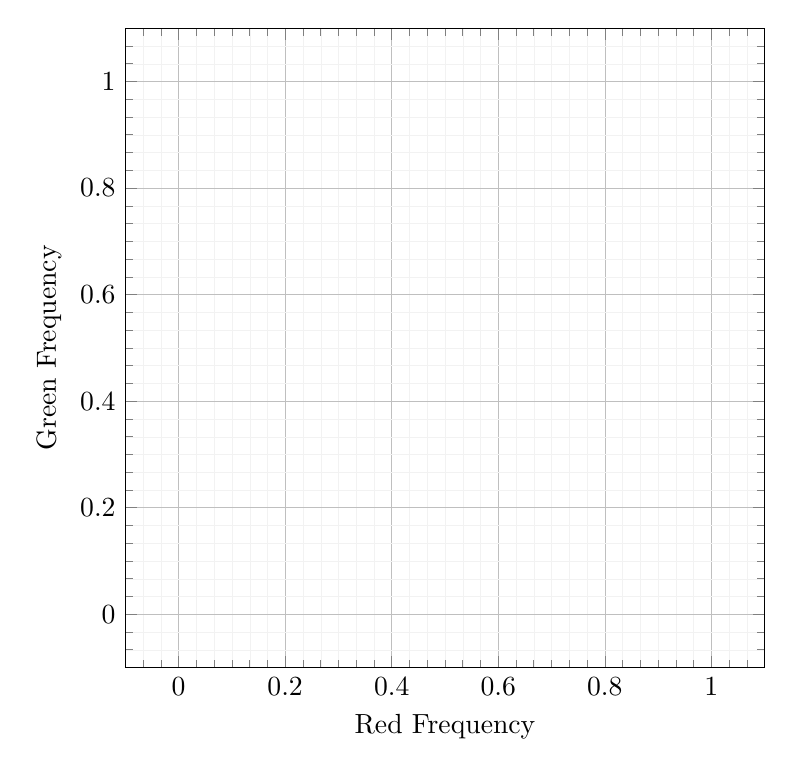
\begin{tikzpicture}
        \begin{axis}[
            xlabel={Red Frequency},
            ylabel={Green Frequency},
            zlabel={Blue Frequency},
            xlabel style={sloped like x axis}, % Make x label follow the x axis
            ylabel style={sloped like y axis}, % Make y label follow the y axis
            zlabel style={sloped}, % Make z label follow the z axis or make it vertical
            legend pos=north west,
            grid=both,
            grid style={line width=.1pt, draw=gray!10},
            major grid style={line width=.2pt,draw=gray!50},
            minor tick num=5,
            width=0.8\textwidth,
            height=0.8\textwidth,
            view={-80}{45}, % Adjust the view angle for better visualization
        ]
        \IfFileExists{code/output_data/color_sensor_calibration/rightColor.csv}{

            % SEEN point
            \addplot3[only marks, ball color=\seencolor, mark=ball, mark size = \ballsize*1.3, draw opacity = 0] coordinates {(\seenx, \seeny, \seenz)};
            \addlegendentry{Frequencies Read by Sensor}

            % CALIBRATION point
            \addlegendentry{Closest Calibration Point \& Used Color}
            \addplot3[only marks, ball color=blue, mark=ball, mark size = \ballsize*1.3, draw opacity = 1, draw= \seencolor, line width = 0.5mm] coordinates {(\calix, \caliy, \caliz)};

            % Line between the two
            \addplot3[ no marks,thick, line width=0.5mm, color=\seencolor, opacity = 1, -latex] coordinates {(\seenx, \seeny, \seenz) (\calix, \caliy, \caliz)};

            % Determine opacity based on sensor

            \addplot3[
                only marks,
                scatter,
                scatter/classes={
                    RED={mark=ball,ball color= red, draw opacity=0, mark size = 0},
                    BLUE={mark=ball,ball color= blue, draw opacity=0, mark size = \ballsize},
                    GREEN={mark=ball,ball color= green, draw opacity=0, mark size = 0},
                    WHITE={mark=ball,ball color= white, draw opacity=0, mark size = 0},
                    BLACK={mark=ball,ball color= black, draw opacity=0, mark size = \ballsize},
                    YELLOW={mark=ball,ball color= yellow, draw opacity=0, mark size = 0}
                },
                scatter src=explicit symbolic,
            ] table[
                x=Red_Freq,
                y=Green_Freq,
                z=Blue_Freq,
                meta = Color,
                col sep=comma,
            ] {code/output_data/color_sensor_calibration/rightColor.csv};

            % Wall histogram on the left
            \addplot3[
                only marks,
                scatter,
                scatter/classes={
                    RED={mark=*,fill=gray, fill opacity=0, draw opacity=0},
                    BLUE={mark=*,fill=gray, fill opacity=\grayopacity, draw opacity=0},
                    GREEN={mark=*,fill=gray, fill opacity=0, draw opacity=0},
                    WHITE={mark=*,fill=gray, fill opacity=0, draw opacity=0},
                    BLACK={mark=*,fill=gray, fill opacity=\grayopacity, draw opacity=0},
                    YELLOW={mark=*,fill=gray, fill opacity=0, draw opacity=0}
                },
                scatter src=explicit symbolic,
            ] table[
                x = Red_Freq,  % This sets the x-coordinate to 0
                y expr = 800,  % This sets the y-coordinate to 0
                z= Blue_Freq,
                meta = Color,
                col sep=comma,
            ] {code/output_data/color_sensor_calibration/rightColor.csv};

            % Wall histogram on the right
            \addplot3[
                only marks,
                scatter,
                scatter/classes={
                    RED={mark=*,fill=gray, fill opacity=0, draw opacity=0},
                    BLUE={mark=*,fill=gray, fill opacity=\grayopacity, draw opacity=0},
                    GREEN={mark=*,fill=gray, fill opacity=0, draw opacity=0},
                    WHITE={mark=*,fill=gray, fill opacity=0, draw opacity=0},
                    BLACK={mark=*,fill=gray, fill opacity=\grayopacity, draw opacity=0},
                    YELLOW={mark=*,fill=gray, fill opacity=0, draw opacity=0}
                },
                scatter src=explicit symbolic,
            ] table[
                x expr = 750,  % This sets the x-coordinate to 0
                y = Green_Freq,  % This sets the y-coordinate to the back wall
                z= Blue_Freq,
                meta = Color,
                col sep=comma,
            ] {code/output_data/color_sensor_calibration/rightColor.csv};

            % Floor histogram
            \addplot3[
                only marks,
                scatter,
                scatter/classes={
                    RED={mark=*,fill=gray, fill opacity=0, draw opacity=0},
                    BLUE={mark=*,fill=gray, fill opacity=\grayopacity, draw opacity=0},
                    GREEN={mark=*,fill=gray, fill opacity=0, draw opacity=0},
                    WHITE={mark=*,fill=gray, fill opacity=0, draw opacity=0},
                    BLACK={mark=*,fill=gray, fill opacity=\grayopacity, draw opacity=0},
                    YELLOW={mark=*,fill=gray, fill opacity=0, draw opacity=0}
                },
                scatter src=explicit symbolic,
            ] table[
                x = Red_Freq,
                y = Green_Freq,
                z expr = 0,
                meta = Color,
                col sep=comma,
            ] {code/output_data/color_sensor_calibration/rightColor.csv};

            
        }{}
        \end{axis}
    \end{tikzpicture}
    \caption{Visual representation of color matching algorithm. The orange dot is the seen color by the sensor, and the nearest calibration point is blue, thus the color seen is set to blue.}
    \label{fig:color-calibration-distance-example}
\end{figure}

\end{document}

            % SEEN point on bottom wall
            \addplot3[only marks, mark = *, fill = \seencolor,fill opacity = \shadowopacity, draw opacity = 0, mark size = \ballsize*0.9] coordinates {(\seenx, \seeny, 0)};

            % CALIBRATION point on bottom wall
            \addplot3[only marks, mark = *, fill = \calicolor,fill opacity = \shadowopacity, draw opacity = 0, mark size = \ballsize*0.9] coordinates {(\calix, \caliy, 0)};

            % Line on bottom wall
            \addplot3[ no marks,thick, line width=0.5mm, color=\seencolor, opacity = \shadowopacity, -latex] coordinates {(\seenx, \seeny, 0) (\calix, \caliy, 0)};

            % SEEN point on right wall
            \addplot3[only marks, mark = *, fill = \seencolor,fill opacity = \shadowopacity, draw opacity = 0, mark size = \ballsize*0.9] coordinates {(\maxx, \seeny, \seenz)};

            % CALIBRATION point on right wall
            \addplot3[only marks, mark = *, fill = \calicolor,fill opacity = \shadowopacity, draw opacity = 0, mark size = \ballsize*0.9] coordinates {(\maxx, \caliy, \caliz)};

            % Line on right wall
            \addplot3[ no marks,thick, line width=0.5mm, color=\seencolor, opacity = \shadowopacity, -latex] coordinates {(\maxx, \seeny, \seenz) (\maxx, \caliy, \caliz)};


\subsection{Design 3}
\section{IR Array Calibration Points}
\label{sc:ir-array-points}
\documentclass{article}
\usepackage{GraphDefinitions}

\begin{document}

\begin{figure}[H]
\centering
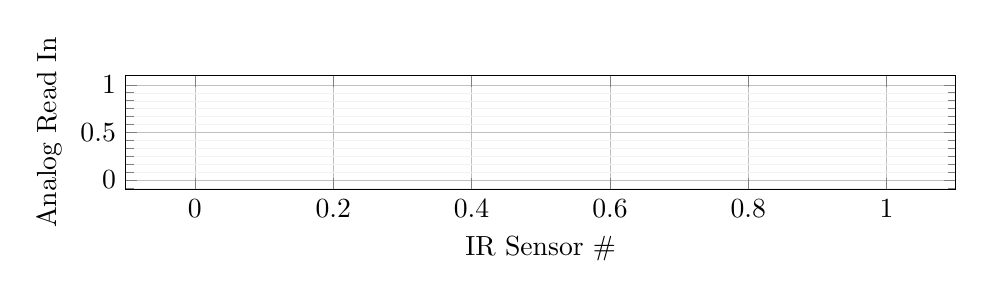
\begin{tikzpicture}
\begin{axis}[
    width=1\textwidth, % Adjust the width as needed
    height=0.25\textwidth, % Adjust the height as needed
    xlabel={IR Sensor \#},
    ylabel={Analog Read In},
    xtick={1, 2, 3, 4, 5, 6, 7}, % Set specific x-axis labels
    legend pos=north west,
    grid=both,
    grid style={line width=.1pt, draw=gray!10},
    major grid style={line width=.2pt,draw=gray!50},
    minor y tick num=5, % This adds the minor grid lines on the y-axis
    minor x tick num=0, % This removes the minor grid lines on the x-axis
    ]
    \IRTrace{green}{Green}{green}
    \IRTrace{blue}{Blue}{blue}
    \IRTrace{red}{Red}{red}
    \IRTrace{yellow}{Yellow}{black}
    \IRTrace{black}{Off}{black}
\end{axis}
\end{tikzpicture}
\caption{IR Calibration Data Based on Tape Color.}
\label{ir-calibration-data}
\end{figure}

\end{document}


\subsection{Design 4}
\section{Motor Calibration Points}
\label{sc:motor-points}
\documentclass[12pt]{report}
\usepackage{GraphDefinitions}

\begin{document}

\begin{figure}[H]
\centering
\begin{tikzpicture}
    \begin{axis}[
        title = {Speed Percent ($\% \cdot 100$) vs Speed (cm/s)}
        width=\textwidth, % Make the plot as wide as the subfigure
        height=0.5\textwidth, % Adjust the height for a wide format
        xlabel={Speed (cm/s)},
        ylabel={Speed Percent ($\% \cdot 100$)},
        legend pos=north west,
        ymin = -10,
        grid=both,
        grid style={line width=.1pt, draw=gray!10},
        major grid style={line width=.2pt,draw=gray!50},
        ]
        \MotorTrace{left}{speed_percent}{Left Speed Percent}{red}{solid}        
        \MotorTrace{right}{speed_percent}{Right Speed Percent}{green}{solid}
        \MotorTrace{top}{speed_percent}{Top Speed Percent}{blue}{solid}
        \MotorTrace{bottom}{speed_percent}{Bottom Speed Percent}{black}{solid}
    \end{axis}
\end{tikzpicture}
\label{speed-calibration-data}
\caption{Motor Calibration Data Regarding Speed Percent}
\end{figure}

\vspace{0.5cm} % Space between the subfigures

\begin{figure}[H]
\centering
\begin{tikzpicture}
    \begin{axis}[
        title = {PWM Percent ($\% \cdot 100$) vs Speed (cm/s)}
        width=\textwidth, % Make the plot as wide as the subfigure
        height=0.5\textwidth, % Adjust the height for a wide format
        xlabel={Speed (cm/s)},
        ylabel={PWM Percent ($\% \cdot 100$)},
        ymin = -10,
        legend pos=north west,
        grid=both,
        grid style={line width=.1pt, draw=gray!10},
        major grid style={line width=.2pt,draw=gray!50},
        ]
        \MotorTrace{left}{pwm_percent}{Left PWM Percent}{red}{solid}        
        \MotorTrace{right}{pwm_percent}{Right PWM Percent}{green}{solid}
        \MotorTrace{top}{pwm_percent}{Top PWM Percent}{blue}{solid}
        \MotorTrace{bottom}{pwm_percent}{Bottom PWM Percent}{black}{solid}
    \end{axis}
\end{tikzpicture}
\label{pwm-calibration-data}
\caption{Motor Calibration Data Regarding PWM Percent}
\end{figure}

\end{document}


\end{document}
\documentclass[12pt]{report}
\usepackage{StyleSheets/main}
\begin{document}

\pagestyle{code} % Removes footer line 
\thispagestyle{code} % Overrides the chapter "plain" style

\chapter{Code}\label{ap:code}

\section{main.ino}
\lstinputlisting[language=cpp,  caption={main.ino}, label=lst:main-h]{code/main/main.ino}


\section{ObstacleAvoidance.h}
\lstinputlisting[language=cpp,  caption={ObstacleAvoidance.h}, label=lst:obstacleavoidance-h]{code/main/ObstacleAvoidance.h}

\section{PickupPlace.h}
\lstinputlisting[language=cpp,  caption={PickupPlace.h}, label=lst:pickupplace-h]{code/main/PickupPlace.h}

\section{Initialization.h}
\lstinputlisting[language=cpp,  caption={Initialization.h}, label=lst:initialization-h]{code/main/Initialization.h}

\section{LineFollowing.h}
\lstinputlisting[language=cpp,  caption={LineFollowing.h}, label=lst:linefollowing-h]{code/main/LineFollowing.h}

\section{Motion.h}
\lstinputlisting[language=cpp,  caption={Motion.h}, label=lst:motion-h]{code/main/Motion.h}

\section{Sensors}

\subsection{Button.h}
\lstinputlisting[language=cpp,  caption={Button.h}, label=lst:button-h]{code/main/sensors/Button.h}

\subsection{ColorSensor.h}
\lstinputlisting[language=cpp,  caption={ColorSensor.h}, label=lst:colorsensor-h]{code/main/sensors/ColorSensor.h}

\subsection{IRSensorArray.h}
\lstinputlisting[language=cpp,  caption={IRSensorArray.h}, label=lst:irsensorarray-h]{code/main/sensors/IRSensorArray.h}

\subsection{Motor.h}
\lstinputlisting[language=cpp,  caption={Motor.h}, label=lst:motor-h]{code/main/sensors/Motor.h}

\subsection{MWServo.h}
\lstinputlisting[language=cpp,  caption={MWServo.h}, label=lst:mwservo-h]{code/main/sensors/MWServo.h}

\subsection{UltraSonic.h}
\lstinputlisting[language=cpp,  caption={UltraSonic.h}, label=lst:ultrasonic-h]{code/main/sensors/UltraSonic.h}

\section{Controls}
\subsection{PIDController.h}
\lstinputlisting[language=cpp,  caption={PIDController.h}, label=lst:pidcontroller-h]{code/main/controls/PIDController.h}

\subsection{Utils.h}
\lstinputlisting[language=cpp,  caption={Utils.h}, label=lst:utils-h]{code/main/controls/Utils.h}

\section{BoxControl.h}
\lstinputlisting[language=cpp,  caption={BoxControl.h}, label=lst:boxcontrol-h]{code/main/BoxControl.h}


\pagestyle{fancy} % Defaults to normal headers & footers

\end{document}


\end{document}